% Options for packages loaded elsewhere
\PassOptionsToPackage{unicode}{hyperref}
\PassOptionsToPackage{hyphens}{url}
%
\documentclass[
]{book}
\usepackage{lmodern}
\usepackage{amssymb,amsmath}
\usepackage{ifxetex,ifluatex}
\ifnum 0\ifxetex 1\fi\ifluatex 1\fi=0 % if pdftex
  \usepackage[T1]{fontenc}
  \usepackage[utf8]{inputenc}
  \usepackage{textcomp} % provide euro and other symbols
\else % if luatex or xetex
  \usepackage{unicode-math}
  \defaultfontfeatures{Scale=MatchLowercase}
  \defaultfontfeatures[\rmfamily]{Ligatures=TeX,Scale=1}
\fi
% Use upquote if available, for straight quotes in verbatim environments
\IfFileExists{upquote.sty}{\usepackage{upquote}}{}
\IfFileExists{microtype.sty}{% use microtype if available
  \usepackage[]{microtype}
  \UseMicrotypeSet[protrusion]{basicmath} % disable protrusion for tt fonts
}{}
\makeatletter
\@ifundefined{KOMAClassName}{% if non-KOMA class
  \IfFileExists{parskip.sty}{%
    \usepackage{parskip}
  }{% else
    \setlength{\parindent}{0pt}
    \setlength{\parskip}{6pt plus 2pt minus 1pt}}
}{% if KOMA class
  \KOMAoptions{parskip=half}}
\makeatother
\usepackage{xcolor}
\IfFileExists{xurl.sty}{\usepackage{xurl}}{} % add URL line breaks if available
\IfFileExists{bookmark.sty}{\usepackage{bookmark}}{\usepackage{hyperref}}
\hypersetup{
  pdftitle={ANN in R},
  pdfauthor={Dr Sebnem Er},
  hidelinks,
  pdfcreator={LaTeX via pandoc}}
\urlstyle{same} % disable monospaced font for URLs
\usepackage{color}
\usepackage{fancyvrb}
\newcommand{\VerbBar}{|}
\newcommand{\VERB}{\Verb[commandchars=\\\{\}]}
\DefineVerbatimEnvironment{Highlighting}{Verbatim}{commandchars=\\\{\}}
% Add ',fontsize=\small' for more characters per line
\usepackage{framed}
\definecolor{shadecolor}{RGB}{248,248,248}
\newenvironment{Shaded}{\begin{snugshade}}{\end{snugshade}}
\newcommand{\AlertTok}[1]{\textcolor[rgb]{0.94,0.16,0.16}{#1}}
\newcommand{\AnnotationTok}[1]{\textcolor[rgb]{0.56,0.35,0.01}{\textbf{\textit{#1}}}}
\newcommand{\AttributeTok}[1]{\textcolor[rgb]{0.77,0.63,0.00}{#1}}
\newcommand{\BaseNTok}[1]{\textcolor[rgb]{0.00,0.00,0.81}{#1}}
\newcommand{\BuiltInTok}[1]{#1}
\newcommand{\CharTok}[1]{\textcolor[rgb]{0.31,0.60,0.02}{#1}}
\newcommand{\CommentTok}[1]{\textcolor[rgb]{0.56,0.35,0.01}{\textit{#1}}}
\newcommand{\CommentVarTok}[1]{\textcolor[rgb]{0.56,0.35,0.01}{\textbf{\textit{#1}}}}
\newcommand{\ConstantTok}[1]{\textcolor[rgb]{0.00,0.00,0.00}{#1}}
\newcommand{\ControlFlowTok}[1]{\textcolor[rgb]{0.13,0.29,0.53}{\textbf{#1}}}
\newcommand{\DataTypeTok}[1]{\textcolor[rgb]{0.13,0.29,0.53}{#1}}
\newcommand{\DecValTok}[1]{\textcolor[rgb]{0.00,0.00,0.81}{#1}}
\newcommand{\DocumentationTok}[1]{\textcolor[rgb]{0.56,0.35,0.01}{\textbf{\textit{#1}}}}
\newcommand{\ErrorTok}[1]{\textcolor[rgb]{0.64,0.00,0.00}{\textbf{#1}}}
\newcommand{\ExtensionTok}[1]{#1}
\newcommand{\FloatTok}[1]{\textcolor[rgb]{0.00,0.00,0.81}{#1}}
\newcommand{\FunctionTok}[1]{\textcolor[rgb]{0.00,0.00,0.00}{#1}}
\newcommand{\ImportTok}[1]{#1}
\newcommand{\InformationTok}[1]{\textcolor[rgb]{0.56,0.35,0.01}{\textbf{\textit{#1}}}}
\newcommand{\KeywordTok}[1]{\textcolor[rgb]{0.13,0.29,0.53}{\textbf{#1}}}
\newcommand{\NormalTok}[1]{#1}
\newcommand{\OperatorTok}[1]{\textcolor[rgb]{0.81,0.36,0.00}{\textbf{#1}}}
\newcommand{\OtherTok}[1]{\textcolor[rgb]{0.56,0.35,0.01}{#1}}
\newcommand{\PreprocessorTok}[1]{\textcolor[rgb]{0.56,0.35,0.01}{\textit{#1}}}
\newcommand{\RegionMarkerTok}[1]{#1}
\newcommand{\SpecialCharTok}[1]{\textcolor[rgb]{0.00,0.00,0.00}{#1}}
\newcommand{\SpecialStringTok}[1]{\textcolor[rgb]{0.31,0.60,0.02}{#1}}
\newcommand{\StringTok}[1]{\textcolor[rgb]{0.31,0.60,0.02}{#1}}
\newcommand{\VariableTok}[1]{\textcolor[rgb]{0.00,0.00,0.00}{#1}}
\newcommand{\VerbatimStringTok}[1]{\textcolor[rgb]{0.31,0.60,0.02}{#1}}
\newcommand{\WarningTok}[1]{\textcolor[rgb]{0.56,0.35,0.01}{\textbf{\textit{#1}}}}
\usepackage{longtable,booktabs}
% Correct order of tables after \paragraph or \subparagraph
\usepackage{etoolbox}
\makeatletter
\patchcmd\longtable{\par}{\if@noskipsec\mbox{}\fi\par}{}{}
\makeatother
% Allow footnotes in longtable head/foot
\IfFileExists{footnotehyper.sty}{\usepackage{footnotehyper}}{\usepackage{footnote}}
\makesavenoteenv{longtable}
\usepackage{graphicx,grffile}
\makeatletter
\def\maxwidth{\ifdim\Gin@nat@width>\linewidth\linewidth\else\Gin@nat@width\fi}
\def\maxheight{\ifdim\Gin@nat@height>\textheight\textheight\else\Gin@nat@height\fi}
\makeatother
% Scale images if necessary, so that they will not overflow the page
% margins by default, and it is still possible to overwrite the defaults
% using explicit options in \includegraphics[width, height, ...]{}
\setkeys{Gin}{width=\maxwidth,height=\maxheight,keepaspectratio}
% Set default figure placement to htbp
\makeatletter
\def\fps@figure{htbp}
\makeatother
\setlength{\emergencystretch}{3em} % prevent overfull lines
\providecommand{\tightlist}{%
  \setlength{\itemsep}{0pt}\setlength{\parskip}{0pt}}
\setcounter{secnumdepth}{5}
\usepackage{booktabs}
\usepackage[]{natbib}
\bibliographystyle{apalike}

\title{ANN in R}
\author{Dr Sebnem Er}
\date{2021-05-20}

\begin{document}
\maketitle

{
\setcounter{tocdepth}{1}
\tableofcontents
}
\hypertarget{introduction}{%
\chapter{Introduction}\label{introduction}}

In this tutorial you will be introduced to several R packages and how to use some of them such as \emph{neuralnet} , \emph{keras} and \emph{h2o} .

In any of these packages the order of NN application is standard:

1 - Preprocess your data:

\begin{itemize}
\item
  Standardize or normalize your data (scale or min-max)
\item
  Missing values, outliers
\item
  Training/Validation and Test set splits
\end{itemize}

2 - Construct your NN model, ie. number of neurons, number of layers, learning rate, regularization etc. (these are your hyperparameters)

3 - Fit your model

4 - Predict your Y variable for both training and validation sets.

5 - Extract the training and validation errors, visualize these for different number of hyperparameters (fine tuning)

6 - Choose the parameters based on the smallest validation error.

7 - Assess the performance of your predicted model on the test set. Remember the test set error is not for decision making!

\hypertarget{neuralnet}{%
\chapter{Neuralnet Package}\label{neuralnet}}

\begin{Shaded}
\begin{Highlighting}[]
\CommentTok{#install.packages("neuralnet")}
\KeywordTok{rm}\NormalTok{(}\DataTypeTok{list=}\KeywordTok{ls}\NormalTok{())}
\KeywordTok{library}\NormalTok{(neuralnet)}
\end{Highlighting}
\end{Shaded}

\hypertarget{example-1---boston}{%
\section{Example 1 - Boston}\label{example-1---boston}}

\begin{Shaded}
\begin{Highlighting}[]
\KeywordTok{library}\NormalTok{(MASS)}
\KeywordTok{rm}\NormalTok{(}\DataTypeTok{list=}\KeywordTok{ls}\NormalTok{())}
\KeywordTok{data}\NormalTok{(Boston)}
\end{Highlighting}
\end{Shaded}

\hypertarget{scale-training-and-test-datasets}{%
\subsection{Scale, Training and Test Datasets}\label{scale-training-and-test-datasets}}

\begin{Shaded}
\begin{Highlighting}[]
\NormalTok{Boston.st =}\StringTok{ }\KeywordTok{scale}\NormalTok{(Boston)}
\KeywordTok{set.seed}\NormalTok{(}\DecValTok{1}\NormalTok{)}
\NormalTok{index <-}\StringTok{ }\KeywordTok{sample}\NormalTok{(}\DecValTok{1}\OperatorTok{:}\KeywordTok{nrow}\NormalTok{(Boston.st),}\KeywordTok{round}\NormalTok{(}\FloatTok{0.8}\OperatorTok{*}\KeywordTok{nrow}\NormalTok{(Boston.st)))}
\NormalTok{trainBoston.st <-}\StringTok{ }\NormalTok{Boston.st[index,]}
\NormalTok{testBoston.st <-}\StringTok{ }\NormalTok{Boston.st[}\OperatorTok{-}\NormalTok{index,]}
\end{Highlighting}
\end{Shaded}

\hypertarget{build-model}{%
\subsection{Build model}\label{build-model}}

\begin{Shaded}
\begin{Highlighting}[]
\KeywordTok{set.seed}\NormalTok{(}\DecValTok{1}\NormalTok{)}
\NormalTok{neuralnetmodel =}\StringTok{ }\KeywordTok{neuralnet}\NormalTok{(medv}\OperatorTok{~}\NormalTok{crim}\OperatorTok{+}\NormalTok{nox, }\DataTypeTok{data =}\NormalTok{ trainBoston.st, }
                           \DataTypeTok{linear.output =} \OtherTok{TRUE}\NormalTok{, }
                           \DataTypeTok{act.fct =} \StringTok{"logistic"}\NormalTok{,}
                           \DataTypeTok{hidden =} \KeywordTok{c}\NormalTok{(}\DecValTok{2}\NormalTok{))}
\end{Highlighting}
\end{Shaded}

\begin{Shaded}
\begin{Highlighting}[]
\KeywordTok{plot}\NormalTok{(neuralnetmodel)}
\end{Highlighting}
\end{Shaded}

\begin{Shaded}
\begin{Highlighting}[]
\NormalTok{neuralnetmodel}\OperatorTok{$}\NormalTok{weights}
\end{Highlighting}
\end{Shaded}

\begin{verbatim}
## [[1]]
## [[1]][[1]]
##            [,1]      [,2]
## [1,]  -38.34128  5.724901
## [2,]   20.11112 -3.802220
## [3,] -122.96637 -2.323184
## 
## [[1]][[2]]
##            [,1]
## [1,] -1.4262287
## [2,]  0.6035351
## [3,]  1.3660896
\end{verbatim}

\begin{Shaded}
\begin{Highlighting}[]
\NormalTok{neuralnetmodel}\OperatorTok{$}\NormalTok{err.fct}
\end{Highlighting}
\end{Shaded}

\begin{verbatim}
## function (x, y) 
## {
##     1/2 * (y - x)^2
## }
## <bytecode: 0x000000001c462b10>
## <environment: 0x0000000021e72378>
## attr(,"type")
## [1] "sse"
\end{verbatim}

\begin{Shaded}
\begin{Highlighting}[]
\NormalTok{neuralnetmodel}\OperatorTok{$}\NormalTok{act.fct}
\end{Highlighting}
\end{Shaded}

\begin{verbatim}
## function (x) 
## {
##     1/(1 + exp(-x))
## }
## <bytecode: 0x000000001c45c288>
## <environment: 0x0000000021e753a8>
## attr(,"type")
## [1] "logistic"
\end{verbatim}

\hypertarget{get-the-predictions-train-set}{%
\subsection{Get the predictions train set}\label{get-the-predictions-train-set}}

\begin{Shaded}
\begin{Highlighting}[]
\NormalTok{train.st.y.predict =}\StringTok{ }\KeywordTok{predict}\NormalTok{(neuralnetmodel,trainBoston.st)}
\KeywordTok{head}\NormalTok{(train.st.y.predict, }\DecValTok{3}\NormalTok{)}
\end{Highlighting}
\end{Shaded}

\begin{verbatim}
##            [,1]
## 505 -0.06150515
## 324  0.54309902
## 167 -0.06612987
\end{verbatim}

\begin{Shaded}
\begin{Highlighting}[]
\DecValTok{1}\OperatorTok{/}\DecValTok{2}\OperatorTok{*}\NormalTok{(}\KeywordTok{sum}\NormalTok{((trainBoston.st[,}\StringTok{"medv"}\NormalTok{]}\OperatorTok{-}\KeywordTok{as.numeric}\NormalTok{(train.st.y.predict))}\OperatorTok{^}\DecValTok{2}\NormalTok{))}
\end{Highlighting}
\end{Shaded}

\begin{verbatim}
## [1] 153.874
\end{verbatim}

\begin{Shaded}
\begin{Highlighting}[]
\CommentTok{#[1] 153.874}
\end{Highlighting}
\end{Shaded}

\begin{Shaded}
\begin{Highlighting}[]
\NormalTok{average.error.train =}\StringTok{ }\DecValTok{1}\OperatorTok{/}\NormalTok{(}\DecValTok{405}\NormalTok{)}\OperatorTok{*}\NormalTok{(}\KeywordTok{sum}\NormalTok{((trainBoston.st[,}\StringTok{"medv"}\NormalTok{]}\OperatorTok{-}\KeywordTok{as.numeric}\NormalTok{(train.st.y.predict))}\OperatorTok{^}\DecValTok{2}\NormalTok{))}
\NormalTok{average.error.train}
\end{Highlighting}
\end{Shaded}

\begin{verbatim}
## [1] 0.7598714
\end{verbatim}

\begin{Shaded}
\begin{Highlighting}[]
\FloatTok{153.874}\OperatorTok{*}\DecValTok{2}\OperatorTok{/}\DecValTok{405}
\end{Highlighting}
\end{Shaded}

\begin{verbatim}
## [1] 0.7598716
\end{verbatim}

\hypertarget{get-the-predictions-test-set}{%
\subsection{Get the predictions test set}\label{get-the-predictions-test-set}}

\begin{Shaded}
\begin{Highlighting}[]
\NormalTok{test.st.y.predict =}\StringTok{ }\KeywordTok{predict}\NormalTok{(neuralnetmodel,testBoston.st)}
\KeywordTok{head}\NormalTok{(test.st.y.predict, }\DecValTok{3}\NormalTok{)}
\end{Highlighting}
\end{Shaded}

\begin{verbatim}
##          [,1]
## 6  0.54326440
## 7 -0.06064561
## 9 -0.06067375
\end{verbatim}

\begin{Shaded}
\begin{Highlighting}[]
\DecValTok{1}\OperatorTok{/}\DecValTok{2}\OperatorTok{*}\NormalTok{(}\KeywordTok{sum}\NormalTok{((testBoston.st[,}\StringTok{"medv"}\NormalTok{]}\OperatorTok{-}\KeywordTok{as.numeric}\NormalTok{(test.st.y.predict))}\OperatorTok{^}\DecValTok{2}\NormalTok{))}
\end{Highlighting}
\end{Shaded}

\begin{verbatim}
## [1] 22.56024
\end{verbatim}

\begin{Shaded}
\begin{Highlighting}[]
\CommentTok{#[1] 22.56024}
\end{Highlighting}
\end{Shaded}

\begin{Shaded}
\begin{Highlighting}[]
\NormalTok{average.error.test =}\StringTok{ }\DecValTok{1}\OperatorTok{/}\NormalTok{(}\DecValTok{101}\NormalTok{)}\OperatorTok{*}\NormalTok{(}\KeywordTok{sum}\NormalTok{((testBoston.st[,}\StringTok{"medv"}\NormalTok{]}\OperatorTok{-}\KeywordTok{as.numeric}\NormalTok{(test.st.y.predict))}\OperatorTok{^}\DecValTok{2}\NormalTok{))}
\NormalTok{average.error.test}
\end{Highlighting}
\end{Shaded}

\begin{verbatim}
## [1] 0.4467374
\end{verbatim}

\hypertarget{forward-propagation}{%
\subsection{Forward propagation}\label{forward-propagation}}

\begin{Shaded}
\begin{Highlighting}[]
\KeywordTok{head}\NormalTok{(trainBoston.st[,}\KeywordTok{c}\NormalTok{(}\StringTok{"crim"}\NormalTok{,}\StringTok{"nox"}\NormalTok{,}\StringTok{"medv"}\NormalTok{)])}
\end{Highlighting}
\end{Shaded}

\begin{verbatim}
##            crim        nox        medv
## 505 -0.40736095  0.1579678 -0.05793197
## 324 -0.38709366 -0.5324154 -0.43848654
## 167 -0.18640065  0.4341211  2.98650460
## 129 -0.38226778  0.5980871 -0.49285148
## 418  2.59570533  1.0727255 -1.31919854
## 471  0.08548074  0.2183763 -0.28626471
\end{verbatim}

\begin{Shaded}
\begin{Highlighting}[]
\NormalTok{trainBoston.st[}\DecValTok{1}\NormalTok{,}\KeywordTok{c}\NormalTok{(}\StringTok{"crim"}\NormalTok{,}\StringTok{"nox"}\NormalTok{,}\StringTok{"medv"}\NormalTok{)]}
\end{Highlighting}
\end{Shaded}

\begin{verbatim}
##        crim         nox        medv 
## -0.40736095  0.15796779 -0.05793197
\end{verbatim}

\begin{Shaded}
\begin{Highlighting}[]
\NormalTok{Z1_}\DecValTok{2}\NormalTok{ =}\StringTok{ }\KeywordTok{sum}\NormalTok{(neuralnetmodel}\OperatorTok{$}\NormalTok{weights[[}\DecValTok{1}\NormalTok{]][[}\DecValTok{1}\NormalTok{]][,}\DecValTok{1}\NormalTok{]}\OperatorTok{*}\KeywordTok{c}\NormalTok{(}\DecValTok{1}\NormalTok{,trainBoston.st[}\DecValTok{1}\NormalTok{,}\KeywordTok{c}\NormalTok{(}\StringTok{"crim"}\NormalTok{,}\StringTok{"nox"}\NormalTok{)]))}
\NormalTok{Z1_}\DecValTok{2}
\end{Highlighting}
\end{Shaded}

\begin{verbatim}
## [1] -65.95849
\end{verbatim}

\begin{Shaded}
\begin{Highlighting}[]
\NormalTok{a1_}\DecValTok{2}\NormalTok{ =}\StringTok{ }\DecValTok{1}\OperatorTok{/}\NormalTok{(}\DecValTok{1}\OperatorTok{+}\KeywordTok{exp}\NormalTok{(}\OperatorTok{-}\NormalTok{Z1_}\DecValTok{2}\NormalTok{))}
\NormalTok{a1_}\DecValTok{2}
\end{Highlighting}
\end{Shaded}

\begin{verbatim}
## [1] 2.26251e-29
\end{verbatim}

\begin{Shaded}
\begin{Highlighting}[]
\NormalTok{Z2_}\DecValTok{2}\NormalTok{ =}\StringTok{ }\KeywordTok{sum}\NormalTok{(neuralnetmodel}\OperatorTok{$}\NormalTok{weights[[}\DecValTok{1}\NormalTok{]][[}\DecValTok{1}\NormalTok{]][,}\DecValTok{2}\NormalTok{]}\OperatorTok{*}\KeywordTok{c}\NormalTok{(}\DecValTok{1}\NormalTok{,trainBoston.st[}\DecValTok{1}\NormalTok{,}\KeywordTok{c}\NormalTok{(}\StringTok{"crim"}\NormalTok{,}\StringTok{"nox"}\NormalTok{)]))}
\NormalTok{Z2_}\DecValTok{2}
\end{Highlighting}
\end{Shaded}

\begin{verbatim}
## [1] 6.906789
\end{verbatim}

\begin{Shaded}
\begin{Highlighting}[]
\NormalTok{a2_}\DecValTok{2}\NormalTok{ =}\StringTok{ }\DecValTok{1}\OperatorTok{/}\NormalTok{(}\DecValTok{1}\OperatorTok{+}\KeywordTok{exp}\NormalTok{(}\OperatorTok{-}\NormalTok{Z2_}\DecValTok{2}\NormalTok{))}
\NormalTok{a2_}\DecValTok{2}
\end{Highlighting}
\end{Shaded}

\begin{verbatim}
## [1] 0.999
\end{verbatim}

\begin{Shaded}
\begin{Highlighting}[]
\NormalTok{Z1_}\DecValTok{3}\NormalTok{ =}\StringTok{ }\KeywordTok{sum}\NormalTok{(neuralnetmodel}\OperatorTok{$}\NormalTok{weights[[}\DecValTok{1}\NormalTok{]][[}\DecValTok{2}\NormalTok{]][,}\DecValTok{1}\NormalTok{]}\OperatorTok{*}\KeywordTok{c}\NormalTok{(}\DecValTok{1}\NormalTok{,a1_}\DecValTok{2}\NormalTok{,a2_}\DecValTok{2}\NormalTok{))}

\NormalTok{a1_}\DecValTok{3}\NormalTok{=Z1_}\DecValTok{3}
\NormalTok{a1_}\DecValTok{3}
\end{Highlighting}
\end{Shaded}

\begin{verbatim}
## [1] -0.06150515
\end{verbatim}

\hypertarget{model-tuning}{%
\subsection{Model Tuning}\label{model-tuning}}

Although these seem like good results this may simply be a result of the
subseted training and testing data so it is important to test the model
performance further. In this example I will perform k-fold cross validation
using 10 folds (10 fold cross validation)

get the validation indeces using the createFolds function provided by the

caret package

\begin{Shaded}
\begin{Highlighting}[]
\CommentTok{#install.packages("caret")}
\KeywordTok{library}\NormalTok{(caret)}
\KeywordTok{set.seed}\NormalTok{(}\DecValTok{1}\NormalTok{)}
\NormalTok{folds <-}\StringTok{ }\KeywordTok{createFolds}\NormalTok{(trainBoston.st[,}\StringTok{"medv"}\NormalTok{], }\DataTypeTok{k =} \DecValTok{10}\NormalTok{)}
\CommentTok{#results is a vector that will contain the average sum error square for each }
\CommentTok{# of the network trainings for the validation set.}
\end{Highlighting}
\end{Shaded}

\begin{Shaded}
\begin{Highlighting}[]
\CommentTok{#errors.cv.number.of.neurons <- c()}

\CommentTok{#for (hidden in 1:2)\{}
\NormalTok{errors.cv.validation <-}\StringTok{ }\KeywordTok{c}\NormalTok{()}
\ControlFlowTok{for}\NormalTok{ (fld }\ControlFlowTok{in}\NormalTok{ folds)\{}
  
  \CommentTok{#train the network (note I have subsetted out the indeces in the validation set)}
  \KeywordTok{set.seed}\NormalTok{(}\DecValTok{1}\NormalTok{)}
\NormalTok{  neuralnetmodel <-}\StringTok{ }\KeywordTok{neuralnet}\NormalTok{(medv}\OperatorTok{~}\NormalTok{crim}\OperatorTok{+}\NormalTok{nox, }\DataTypeTok{data =}\NormalTok{ trainBoston.st[}\OperatorTok{-}\NormalTok{fld,], }
                  \DataTypeTok{linear.output =} \OtherTok{TRUE}\NormalTok{, }
                  \DataTypeTok{act.fct =} \StringTok{"logistic"}\NormalTok{,}
                  \DataTypeTok{hidden =} \KeywordTok{c}\NormalTok{(}\DecValTok{2}\NormalTok{))}
  
  \CommentTok{#get the predictions from the network for the validation set}
\NormalTok{  yhat.fld <-}\StringTok{ }\KeywordTok{predict}\NormalTok{(neuralnetmodel, trainBoston.st[fld,])}
  
\NormalTok{  errorsq.fld =}\StringTok{ }\NormalTok{(trainBoston.st[fld,}\StringTok{"medv"}\NormalTok{]}\OperatorTok{-}
\StringTok{                                                }\KeywordTok{as.numeric}\NormalTok{(yhat.fld))}\OperatorTok{^}\DecValTok{2}
  
\NormalTok{  errors.cv.validation <-}\StringTok{ }\KeywordTok{c}\NormalTok{(errors.cv.validation, errorsq.fld)}
\NormalTok{\} }

\CommentTok{#errors.cv.number.of.neurons[hidden] = }

\KeywordTok{sum}\NormalTok{(errors.cv.validation)}\OperatorTok{/}\KeywordTok{dim}\NormalTok{(trainBoston.st)[}\DecValTok{1}\NormalTok{]}
\end{Highlighting}
\end{Shaded}

\begin{verbatim}
## [1] 0.7712774
\end{verbatim}

\hypertarget{example-2---iris-dataset}{%
\section{Example 2 - Iris Dataset}\label{example-2---iris-dataset}}

\begin{Shaded}
\begin{Highlighting}[]
\KeywordTok{rm}\NormalTok{(}\DataTypeTok{list=}\KeywordTok{ls}\NormalTok{())}

\KeywordTok{set.seed}\NormalTok{(}\DecValTok{1}\NormalTok{)}
\NormalTok{index <-}\StringTok{ }\KeywordTok{sample}\NormalTok{(}\DecValTok{1}\OperatorTok{:}\KeywordTok{nrow}\NormalTok{(iris),}\KeywordTok{round}\NormalTok{(}\FloatTok{0.8}\OperatorTok{*}\KeywordTok{nrow}\NormalTok{(iris)))}
\NormalTok{trainiris <-}\StringTok{ }\NormalTok{iris[index,]}
\NormalTok{testiris <-}\StringTok{ }\NormalTok{iris[}\OperatorTok{-}\NormalTok{index,]}
\end{Highlighting}
\end{Shaded}

\begin{Shaded}
\begin{Highlighting}[]
\KeywordTok{set.seed}\NormalTok{(}\DecValTok{1}\NormalTok{)}
\NormalTok{neuralnetmodel =}\StringTok{ }\KeywordTok{neuralnet}\NormalTok{(Species}\OperatorTok{~}\NormalTok{Petal.Length}\OperatorTok{+}\NormalTok{Petal.Width, }\DataTypeTok{data =}\NormalTok{ trainiris, }
                           \DataTypeTok{linear.output =} \OtherTok{FALSE}\NormalTok{, }
                           \DataTypeTok{act.fct =} \StringTok{"logistic"}\NormalTok{,}
                           \DataTypeTok{hidden =} \KeywordTok{c}\NormalTok{(}\DecValTok{2}\NormalTok{), }\DataTypeTok{err.fct =} \StringTok{"ce"}\NormalTok{)}
\CommentTok{# stepmax = 1000000, threshold = 0.001, rep = 10 values can be changed as well.}
\end{Highlighting}
\end{Shaded}

\begin{Shaded}
\begin{Highlighting}[]
\KeywordTok{plot}\NormalTok{(neuralnetmodel)}
\end{Highlighting}
\end{Shaded}

\begin{Shaded}
\begin{Highlighting}[]
\NormalTok{neuralnetmodel}\OperatorTok{$}\NormalTok{weights}
\end{Highlighting}
\end{Shaded}

\begin{verbatim}
## [[1]]
## [[1]][[1]]
##           [,1]       [,2]
## [1,]  9.189152 -124.80564
## [2,] -1.436100   33.13635
## [3,] -1.300787   52.19249
## 
## [[1]][[2]]
##            [,1]      [,2]       [,3]
## [1,]   -2.83673 -38.59970   4.022241
## [2,]   39.67766  28.62683 -28.834230
## [3,] -113.70312  24.75467   9.921314
\end{verbatim}

\begin{Shaded}
\begin{Highlighting}[]
\NormalTok{neuralnetmodel}\OperatorTok{$}\NormalTok{err.fct}
\end{Highlighting}
\end{Shaded}

\begin{verbatim}
## function (x, y) 
## {
##     -(y * log(x) + (1 - y) * log(1 - x))
## }
## <bytecode: 0x000000001c4622f8>
## <environment: 0x000000005f2a5bf8>
## attr(,"type")
## [1] "ce"
\end{verbatim}

\begin{Shaded}
\begin{Highlighting}[]
\NormalTok{neuralnetmodel}\OperatorTok{$}\NormalTok{act.fct}
\end{Highlighting}
\end{Shaded}

\begin{verbatim}
## function (x) 
## {
##     1/(1 + exp(-x))
## }
## <bytecode: 0x000000001c45c288>
## <environment: 0x000000005f2a5760>
## attr(,"type")
## [1] "logistic"
\end{verbatim}

\begin{Shaded}
\begin{Highlighting}[]
\NormalTok{train.iris.predict =}\StringTok{ }\KeywordTok{predict}\NormalTok{(neuralnetmodel, trainiris)}
\KeywordTok{head}\NormalTok{(}\KeywordTok{round}\NormalTok{(train.iris.predict,}\DecValTok{3}\NormalTok{), }\DecValTok{3}\NormalTok{)}
\end{Highlighting}
\end{Shaded}

\begin{verbatim}
##     [,1] [,2] [,3]
## 68     0    1    0
## 129    0    0    1
## 43     1    0    0
\end{verbatim}

\begin{Shaded}
\begin{Highlighting}[]
\NormalTok{maxprobability <-}\StringTok{ }\KeywordTok{apply}\NormalTok{(train.iris.predict, }\DecValTok{1}\NormalTok{, which.max) }
\NormalTok{train.iris.predict.class <-}\StringTok{ }\KeywordTok{c}\NormalTok{(}\StringTok{'setosa'}\NormalTok{, }\StringTok{'versicolor'}\NormalTok{, }\StringTok{'virginica'}\NormalTok{)[maxprobability] }
\KeywordTok{head}\NormalTok{(train.iris.predict.class)}
\end{Highlighting}
\end{Shaded}

\begin{verbatim}
## [1] "versicolor" "virginica"  "setosa"     "setosa"     "versicolor"
## [6] "versicolor"
\end{verbatim}

\begin{Shaded}
\begin{Highlighting}[]
\KeywordTok{table}\NormalTok{(train.iris.predict.class, trainiris}\OperatorTok{$}\NormalTok{Species) }
\end{Highlighting}
\end{Shaded}

\begin{verbatim}
##                         
## train.iris.predict.class setosa versicolor virginica
##               setosa         39          0         0
##               versicolor      0         36         2
##               virginica       0          2        41
\end{verbatim}

\begin{Shaded}
\begin{Highlighting}[]
\KeywordTok{mean}\NormalTok{(train.iris.predict.class}\OperatorTok{==}\StringTok{ }\NormalTok{trainiris}\OperatorTok{$}\NormalTok{Species)}\OperatorTok{*}\DecValTok{100}
\end{Highlighting}
\end{Shaded}

\begin{verbatim}
## [1] 96.66667
\end{verbatim}

\begin{Shaded}
\begin{Highlighting}[]
\NormalTok{test.iris.predict =}\StringTok{ }\KeywordTok{predict}\NormalTok{(neuralnetmodel, testiris)}
\KeywordTok{head}\NormalTok{(}\KeywordTok{round}\NormalTok{(train.iris.predict,}\DecValTok{3}\NormalTok{), }\DecValTok{3}\NormalTok{)}
\end{Highlighting}
\end{Shaded}

\begin{verbatim}
##     [,1] [,2] [,3]
## 68     0    1    0
## 129    0    0    1
## 43     1    0    0
\end{verbatim}

\begin{Shaded}
\begin{Highlighting}[]
\NormalTok{maxprobability <-}\StringTok{ }\KeywordTok{apply}\NormalTok{(test.iris.predict, }\DecValTok{1}\NormalTok{, which.max) }
\NormalTok{test.iris.predict.class <-}\StringTok{ }\KeywordTok{c}\NormalTok{(}\StringTok{'setosa'}\NormalTok{, }\StringTok{'versicolor'}\NormalTok{, }\StringTok{'virginica'}\NormalTok{)[maxprobability] }
\KeywordTok{head}\NormalTok{(test.iris.predict.class)}
\end{Highlighting}
\end{Shaded}

\begin{verbatim}
## [1] "setosa" "setosa" "setosa" "setosa" "setosa" "setosa"
\end{verbatim}

\begin{Shaded}
\begin{Highlighting}[]
\KeywordTok{table}\NormalTok{(test.iris.predict.class, testiris}\OperatorTok{$}\NormalTok{Species) }
\end{Highlighting}
\end{Shaded}

\begin{verbatim}
##                        
## test.iris.predict.class setosa versicolor virginica
##              setosa         11          0         0
##              versicolor      0         12         2
##              virginica       0          0         5
\end{verbatim}

\begin{Shaded}
\begin{Highlighting}[]
\KeywordTok{mean}\NormalTok{(test.iris.predict.class}\OperatorTok{==}\StringTok{ }\NormalTok{testiris}\OperatorTok{$}\NormalTok{Species)}\OperatorTok{*}\DecValTok{100}
\end{Highlighting}
\end{Shaded}

\begin{verbatim}
## [1] 93.33333
\end{verbatim}

\hypertarget{model-tuning-1}{%
\subsection{Model Tuning}\label{model-tuning-1}}

Get the validation indices using the createFolds function provided by the caret package

\begin{Shaded}
\begin{Highlighting}[]
\KeywordTok{set.seed}\NormalTok{(}\DecValTok{1}\NormalTok{)}
\NormalTok{folds <-}\StringTok{ }\KeywordTok{createFolds}\NormalTok{(iris}\OperatorTok{$}\NormalTok{Species, }\DataTypeTok{k =} \DecValTok{10}\NormalTok{)}
\CommentTok{#results is a vector that will contain the accuracy for each of the network trainings and testing}
\NormalTok{results <-}\StringTok{ }\KeywordTok{c}\NormalTok{()}
\ControlFlowTok{for}\NormalTok{ (fld }\ControlFlowTok{in}\NormalTok{ folds)\{}
  \CommentTok{#train the network}
  \KeywordTok{set.seed}\NormalTok{(}\DecValTok{1}\NormalTok{)}
\NormalTok{  nn <-}\StringTok{ }\KeywordTok{neuralnet}\NormalTok{(Species}\OperatorTok{~}\NormalTok{Petal.Length}\OperatorTok{+}\NormalTok{Petal.Width, }\DataTypeTok{data =}\NormalTok{ iris[}\OperatorTok{-}\NormalTok{fld,],}
                  \DataTypeTok{hidden =} \KeywordTok{c}\NormalTok{(}\DecValTok{2}\NormalTok{), }\DataTypeTok{err.fct =} \StringTok{"ce"}\NormalTok{, }\DataTypeTok{act.fct =} \StringTok{"logistic"}\NormalTok{,}
                  \DataTypeTok{linear.output =} \OtherTok{FALSE}\NormalTok{, }\DataTypeTok{stepmax =} \DecValTok{1000000}\NormalTok{)}
  
  \CommentTok{#get the classifications from the network}
\NormalTok{  classes <-}\StringTok{ }\KeywordTok{predict}\NormalTok{(nn, iris[fld,])}
\NormalTok{  maxprobability <-}\StringTok{ }\KeywordTok{apply}\NormalTok{(classes, }\DecValTok{1}\NormalTok{, which.max) }
\NormalTok{  valid.iris.predict.class <-}\StringTok{ }\KeywordTok{c}\NormalTok{(}\StringTok{'setosa'}\NormalTok{, }\StringTok{'versicolor'}\NormalTok{, }\StringTok{'virginica'}\NormalTok{)[maxprobability] }
  
\NormalTok{  results <-}\StringTok{ }\KeywordTok{c}\NormalTok{(results, valid.iris.predict.class}\OperatorTok{==}\StringTok{ }\NormalTok{iris[fld,}\StringTok{"Species"}\NormalTok{])}
\NormalTok{\} }

\NormalTok{results}
\end{Highlighting}
\end{Shaded}

\begin{verbatim}
##   [1]  TRUE  TRUE  TRUE  TRUE  TRUE  TRUE  TRUE  TRUE  TRUE  TRUE  TRUE  TRUE
##  [13]  TRUE  TRUE  TRUE  TRUE  TRUE  TRUE  TRUE  TRUE  TRUE  TRUE  TRUE  TRUE
##  [25]  TRUE  TRUE  TRUE  TRUE  TRUE  TRUE  TRUE  TRUE  TRUE  TRUE  TRUE  TRUE
##  [37]  TRUE  TRUE  TRUE  TRUE FALSE  TRUE  TRUE  TRUE  TRUE  TRUE  TRUE  TRUE
##  [49]  TRUE  TRUE  TRUE FALSE  TRUE  TRUE  TRUE  TRUE  TRUE  TRUE  TRUE  TRUE
##  [61]  TRUE  TRUE  TRUE  TRUE  TRUE  TRUE FALSE  TRUE  TRUE  TRUE  TRUE  TRUE
##  [73]  TRUE  TRUE  TRUE  TRUE  TRUE  TRUE  TRUE  TRUE  TRUE  TRUE  TRUE  TRUE
##  [85]  TRUE  TRUE  TRUE  TRUE FALSE  TRUE  TRUE  TRUE  TRUE  TRUE  TRUE  TRUE
##  [97]  TRUE  TRUE FALSE  TRUE  TRUE  TRUE FALSE  TRUE  TRUE  TRUE  TRUE  TRUE
## [109]  TRUE  TRUE  TRUE  TRUE  TRUE  TRUE  TRUE  TRUE  TRUE  TRUE  TRUE  TRUE
## [121]  TRUE  TRUE  TRUE  TRUE  TRUE  TRUE  TRUE  TRUE  TRUE  TRUE  TRUE  TRUE
## [133]  TRUE  TRUE  TRUE  TRUE  TRUE  TRUE  TRUE  TRUE  TRUE  TRUE  TRUE  TRUE
## [145]  TRUE  TRUE  TRUE  TRUE  TRUE  TRUE
\end{verbatim}

\begin{Shaded}
\begin{Highlighting}[]
\KeywordTok{sum}\NormalTok{(results)}\OperatorTok{/}\KeywordTok{length}\NormalTok{(results)}
\end{Highlighting}
\end{Shaded}

\begin{verbatim}
## [1] 0.96
\end{verbatim}

You can label chapter and section titles using \texttt{\{\#label\}} after them, e.g., we can reference Chapter \ref{neuralnet}. If you do not manually label them, there will be automatic labels anyway, e.g., Chapter \ref{keras}.

Figures and tables with captions will be placed in \texttt{figure} and \texttt{table} environments, respectively.

\begin{Shaded}
\begin{Highlighting}[]
\KeywordTok{par}\NormalTok{(}\DataTypeTok{mar =} \KeywordTok{c}\NormalTok{(}\DecValTok{4}\NormalTok{, }\DecValTok{4}\NormalTok{, }\FloatTok{.1}\NormalTok{, }\FloatTok{.1}\NormalTok{))}
\KeywordTok{plot}\NormalTok{(pressure, }\DataTypeTok{type =} \StringTok{'b'}\NormalTok{, }\DataTypeTok{pch =} \DecValTok{19}\NormalTok{)}
\end{Highlighting}
\end{Shaded}

\begin{figure}

{\centering 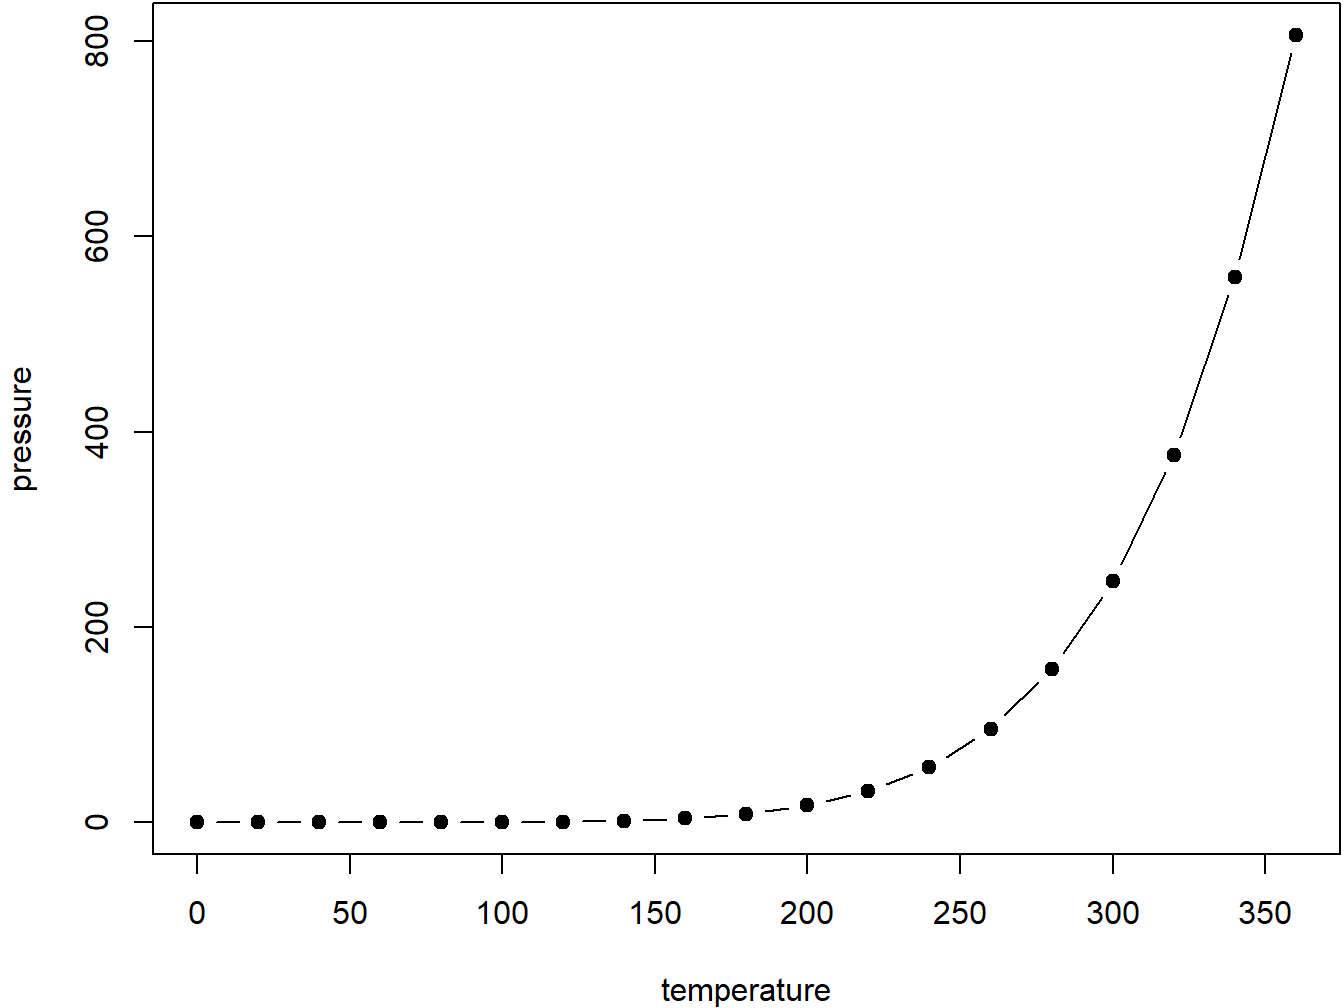
\includegraphics[width=0.8\linewidth]{Keras_files/figure-latex/nice-fig-1} 

}

\caption{Here is a nice figure!}\label{fig:nice-fig}
\end{figure}

Reference a figure by its code chunk label with the \texttt{fig:} prefix, e.g., see Figure \ref{fig:nice-fig}. Similarly, you can reference tables generated from \texttt{knitr::kable()}, e.g., see Table \ref{tab:nice-tab}.

\begin{Shaded}
\begin{Highlighting}[]
\NormalTok{knitr}\OperatorTok{::}\KeywordTok{kable}\NormalTok{(}
  \KeywordTok{head}\NormalTok{(iris, }\DecValTok{20}\NormalTok{), }\DataTypeTok{caption =} \StringTok{'Here is a nice table!'}\NormalTok{,}
  \DataTypeTok{booktabs =} \OtherTok{TRUE}
\NormalTok{)}
\end{Highlighting}
\end{Shaded}

\begin{table}

\caption{\label{tab:nice-tab}Here is a nice table!}
\centering
\begin{tabular}[t]{rrrrl}
\toprule
Sepal.Length & Sepal.Width & Petal.Length & Petal.Width & Species\\
\midrule
5.1 & 3.5 & 1.4 & 0.2 & setosa\\
4.9 & 3.0 & 1.4 & 0.2 & setosa\\
4.7 & 3.2 & 1.3 & 0.2 & setosa\\
4.6 & 3.1 & 1.5 & 0.2 & setosa\\
5.0 & 3.6 & 1.4 & 0.2 & setosa\\
\addlinespace
5.4 & 3.9 & 1.7 & 0.4 & setosa\\
4.6 & 3.4 & 1.4 & 0.3 & setosa\\
5.0 & 3.4 & 1.5 & 0.2 & setosa\\
4.4 & 2.9 & 1.4 & 0.2 & setosa\\
4.9 & 3.1 & 1.5 & 0.1 & setosa\\
\addlinespace
5.4 & 3.7 & 1.5 & 0.2 & setosa\\
4.8 & 3.4 & 1.6 & 0.2 & setosa\\
4.8 & 3.0 & 1.4 & 0.1 & setosa\\
4.3 & 3.0 & 1.1 & 0.1 & setosa\\
5.8 & 4.0 & 1.2 & 0.2 & setosa\\
\addlinespace
5.7 & 4.4 & 1.5 & 0.4 & setosa\\
5.4 & 3.9 & 1.3 & 0.4 & setosa\\
5.1 & 3.5 & 1.4 & 0.3 & setosa\\
5.7 & 3.8 & 1.7 & 0.3 & setosa\\
5.1 & 3.8 & 1.5 & 0.3 & setosa\\
\bottomrule
\end{tabular}
\end{table}

You can write citations, too. For example, we are using the \textbf{bookdown} package \citep{R-bookdown} in this sample book, which was built on top of R Markdown and \textbf{knitr} \citep{xie2015}.

\hypertarget{h2o}{%
\chapter{H2O}\label{h2o}}

H2O is probably the easiest to learn and use.

\begin{Shaded}
\begin{Highlighting}[]
\CommentTok{## Load all packages first}
\KeywordTok{library}\NormalTok{(h2o)}
\KeywordTok{library}\NormalTok{(caret)}
\KeywordTok{library}\NormalTok{(mlbench)}
\KeywordTok{library}\NormalTok{(ggplot2)}
\KeywordTok{library}\NormalTok{(reshape2)}
\KeywordTok{library}\NormalTok{(DEEPR)}

\CommentTok{# http://blog.revolutionanalytics.com/2014/04/a-dive-into-h2o.html}
\CommentTok{# https://discuss.analyticsvidhya.com/t/script-in-h2o-in-r-to-get-you-into-top-30-percentile-for-the-digit-recognizer-competition/6651/8}
\end{Highlighting}
\end{Shaded}

\hypertarget{initialise-h2o-connection}{%
\section{Initialise H2O Connection}\label{initialise-h2o-connection}}

\begin{Shaded}
\begin{Highlighting}[]
\CommentTok{## Start a local H2O cluster directly from R}
\NormalTok{localH2O =}\StringTok{ }\KeywordTok{h2o.init}\NormalTok{(}\DataTypeTok{ip =} \StringTok{"localhost"}\NormalTok{, }\DataTypeTok{port =} \DecValTok{54321}\NormalTok{, }\DataTypeTok{startH2O =} \OtherTok{TRUE}\NormalTok{,}\DataTypeTok{min_mem_size =} \StringTok{"3g"}\NormalTok{)}
\end{Highlighting}
\end{Shaded}

\begin{verbatim}
##  Connection successful!
## 
## R is connected to the H2O cluster: 
##     H2O cluster uptime:         1 hours 1 minutes 
##     H2O cluster timezone:       Africa/Johannesburg 
##     H2O data parsing timezone:  UTC 
##     H2O cluster version:        3.32.0.1 
##     H2O cluster version age:    7 months and 11 days !!! 
##     H2O cluster name:           H2O_started_from_R_01438475_sup231 
##     H2O cluster total nodes:    1 
##     H2O cluster total memory:   3.89 GB 
##     H2O cluster total cores:    4 
##     H2O cluster allowed cores:  4 
##     H2O cluster healthy:        TRUE 
##     H2O Connection ip:          localhost 
##     H2O Connection port:        54321 
##     H2O Connection proxy:       NA 
##     H2O Internal Security:      FALSE 
##     H2O API Extensions:         Amazon S3, Algos, AutoML, Core V3, TargetEncoder, Core V4 
##     R Version:                  R version 4.0.1 (2020-06-06)
\end{verbatim}

\begin{verbatim}
## Warning in h2o.clusterInfo(): 
## Your H2O cluster version is too old (7 months and 11 days)!
## Please download and install the latest version from http://h2o.ai/download/
\end{verbatim}

\begin{Shaded}
\begin{Highlighting}[]
\CommentTok{#Get help}
\NormalTok{?h2o.deeplearning}
\end{Highlighting}
\end{Shaded}

\hypertarget{data-in-h2o-format}{%
\section{Data in H2o format}\label{data-in-h2o-format}}

\begin{Shaded}
\begin{Highlighting}[]
\CommentTok{# iris data ####}
\NormalTok{iris}
\end{Highlighting}
\end{Shaded}

\begin{verbatim}
##     Sepal.Length Sepal.Width Petal.Length Petal.Width    Species
## 1            5.1         3.5          1.4         0.2     setosa
## 2            4.9         3.0          1.4         0.2     setosa
## 3            4.7         3.2          1.3         0.2     setosa
## 4            4.6         3.1          1.5         0.2     setosa
## 5            5.0         3.6          1.4         0.2     setosa
## 6            5.4         3.9          1.7         0.4     setosa
## 7            4.6         3.4          1.4         0.3     setosa
## 8            5.0         3.4          1.5         0.2     setosa
## 9            4.4         2.9          1.4         0.2     setosa
## 10           4.9         3.1          1.5         0.1     setosa
## 11           5.4         3.7          1.5         0.2     setosa
## 12           4.8         3.4          1.6         0.2     setosa
## 13           4.8         3.0          1.4         0.1     setosa
## 14           4.3         3.0          1.1         0.1     setosa
## 15           5.8         4.0          1.2         0.2     setosa
## 16           5.7         4.4          1.5         0.4     setosa
## 17           5.4         3.9          1.3         0.4     setosa
## 18           5.1         3.5          1.4         0.3     setosa
## 19           5.7         3.8          1.7         0.3     setosa
## 20           5.1         3.8          1.5         0.3     setosa
## 21           5.4         3.4          1.7         0.2     setosa
## 22           5.1         3.7          1.5         0.4     setosa
## 23           4.6         3.6          1.0         0.2     setosa
## 24           5.1         3.3          1.7         0.5     setosa
## 25           4.8         3.4          1.9         0.2     setosa
## 26           5.0         3.0          1.6         0.2     setosa
## 27           5.0         3.4          1.6         0.4     setosa
## 28           5.2         3.5          1.5         0.2     setosa
## 29           5.2         3.4          1.4         0.2     setosa
## 30           4.7         3.2          1.6         0.2     setosa
## 31           4.8         3.1          1.6         0.2     setosa
## 32           5.4         3.4          1.5         0.4     setosa
## 33           5.2         4.1          1.5         0.1     setosa
## 34           5.5         4.2          1.4         0.2     setosa
## 35           4.9         3.1          1.5         0.2     setosa
## 36           5.0         3.2          1.2         0.2     setosa
## 37           5.5         3.5          1.3         0.2     setosa
## 38           4.9         3.6          1.4         0.1     setosa
## 39           4.4         3.0          1.3         0.2     setosa
## 40           5.1         3.4          1.5         0.2     setosa
## 41           5.0         3.5          1.3         0.3     setosa
## 42           4.5         2.3          1.3         0.3     setosa
## 43           4.4         3.2          1.3         0.2     setosa
## 44           5.0         3.5          1.6         0.6     setosa
## 45           5.1         3.8          1.9         0.4     setosa
## 46           4.8         3.0          1.4         0.3     setosa
## 47           5.1         3.8          1.6         0.2     setosa
## 48           4.6         3.2          1.4         0.2     setosa
## 49           5.3         3.7          1.5         0.2     setosa
## 50           5.0         3.3          1.4         0.2     setosa
## 51           7.0         3.2          4.7         1.4 versicolor
## 52           6.4         3.2          4.5         1.5 versicolor
## 53           6.9         3.1          4.9         1.5 versicolor
## 54           5.5         2.3          4.0         1.3 versicolor
## 55           6.5         2.8          4.6         1.5 versicolor
## 56           5.7         2.8          4.5         1.3 versicolor
## 57           6.3         3.3          4.7         1.6 versicolor
## 58           4.9         2.4          3.3         1.0 versicolor
## 59           6.6         2.9          4.6         1.3 versicolor
## 60           5.2         2.7          3.9         1.4 versicolor
## 61           5.0         2.0          3.5         1.0 versicolor
## 62           5.9         3.0          4.2         1.5 versicolor
## 63           6.0         2.2          4.0         1.0 versicolor
## 64           6.1         2.9          4.7         1.4 versicolor
## 65           5.6         2.9          3.6         1.3 versicolor
## 66           6.7         3.1          4.4         1.4 versicolor
## 67           5.6         3.0          4.5         1.5 versicolor
## 68           5.8         2.7          4.1         1.0 versicolor
## 69           6.2         2.2          4.5         1.5 versicolor
## 70           5.6         2.5          3.9         1.1 versicolor
## 71           5.9         3.2          4.8         1.8 versicolor
## 72           6.1         2.8          4.0         1.3 versicolor
## 73           6.3         2.5          4.9         1.5 versicolor
## 74           6.1         2.8          4.7         1.2 versicolor
## 75           6.4         2.9          4.3         1.3 versicolor
## 76           6.6         3.0          4.4         1.4 versicolor
## 77           6.8         2.8          4.8         1.4 versicolor
## 78           6.7         3.0          5.0         1.7 versicolor
## 79           6.0         2.9          4.5         1.5 versicolor
## 80           5.7         2.6          3.5         1.0 versicolor
## 81           5.5         2.4          3.8         1.1 versicolor
## 82           5.5         2.4          3.7         1.0 versicolor
## 83           5.8         2.7          3.9         1.2 versicolor
## 84           6.0         2.7          5.1         1.6 versicolor
## 85           5.4         3.0          4.5         1.5 versicolor
## 86           6.0         3.4          4.5         1.6 versicolor
## 87           6.7         3.1          4.7         1.5 versicolor
## 88           6.3         2.3          4.4         1.3 versicolor
## 89           5.6         3.0          4.1         1.3 versicolor
## 90           5.5         2.5          4.0         1.3 versicolor
## 91           5.5         2.6          4.4         1.2 versicolor
## 92           6.1         3.0          4.6         1.4 versicolor
## 93           5.8         2.6          4.0         1.2 versicolor
## 94           5.0         2.3          3.3         1.0 versicolor
## 95           5.6         2.7          4.2         1.3 versicolor
## 96           5.7         3.0          4.2         1.2 versicolor
## 97           5.7         2.9          4.2         1.3 versicolor
## 98           6.2         2.9          4.3         1.3 versicolor
## 99           5.1         2.5          3.0         1.1 versicolor
## 100          5.7         2.8          4.1         1.3 versicolor
## 101          6.3         3.3          6.0         2.5  virginica
## 102          5.8         2.7          5.1         1.9  virginica
## 103          7.1         3.0          5.9         2.1  virginica
## 104          6.3         2.9          5.6         1.8  virginica
## 105          6.5         3.0          5.8         2.2  virginica
## 106          7.6         3.0          6.6         2.1  virginica
## 107          4.9         2.5          4.5         1.7  virginica
## 108          7.3         2.9          6.3         1.8  virginica
## 109          6.7         2.5          5.8         1.8  virginica
## 110          7.2         3.6          6.1         2.5  virginica
## 111          6.5         3.2          5.1         2.0  virginica
## 112          6.4         2.7          5.3         1.9  virginica
## 113          6.8         3.0          5.5         2.1  virginica
## 114          5.7         2.5          5.0         2.0  virginica
## 115          5.8         2.8          5.1         2.4  virginica
## 116          6.4         3.2          5.3         2.3  virginica
## 117          6.5         3.0          5.5         1.8  virginica
## 118          7.7         3.8          6.7         2.2  virginica
## 119          7.7         2.6          6.9         2.3  virginica
## 120          6.0         2.2          5.0         1.5  virginica
## 121          6.9         3.2          5.7         2.3  virginica
## 122          5.6         2.8          4.9         2.0  virginica
## 123          7.7         2.8          6.7         2.0  virginica
## 124          6.3         2.7          4.9         1.8  virginica
## 125          6.7         3.3          5.7         2.1  virginica
## 126          7.2         3.2          6.0         1.8  virginica
## 127          6.2         2.8          4.8         1.8  virginica
## 128          6.1         3.0          4.9         1.8  virginica
## 129          6.4         2.8          5.6         2.1  virginica
## 130          7.2         3.0          5.8         1.6  virginica
## 131          7.4         2.8          6.1         1.9  virginica
## 132          7.9         3.8          6.4         2.0  virginica
## 133          6.4         2.8          5.6         2.2  virginica
## 134          6.3         2.8          5.1         1.5  virginica
## 135          6.1         2.6          5.6         1.4  virginica
## 136          7.7         3.0          6.1         2.3  virginica
## 137          6.3         3.4          5.6         2.4  virginica
## 138          6.4         3.1          5.5         1.8  virginica
## 139          6.0         3.0          4.8         1.8  virginica
## 140          6.9         3.1          5.4         2.1  virginica
## 141          6.7         3.1          5.6         2.4  virginica
## 142          6.9         3.1          5.1         2.3  virginica
## 143          5.8         2.7          5.1         1.9  virginica
## 144          6.8         3.2          5.9         2.3  virginica
## 145          6.7         3.3          5.7         2.5  virginica
## 146          6.7         3.0          5.2         2.3  virginica
## 147          6.3         2.5          5.0         1.9  virginica
## 148          6.5         3.0          5.2         2.0  virginica
## 149          6.2         3.4          5.4         2.3  virginica
## 150          5.9         3.0          5.1         1.8  virginica
\end{verbatim}

\begin{Shaded}
\begin{Highlighting}[]
\NormalTok{index <-}\StringTok{ }\KeywordTok{c}\NormalTok{(}\KeywordTok{sample}\NormalTok{(}\DecValTok{1}\OperatorTok{:}\DecValTok{50}\NormalTok{,}\DecValTok{25}\NormalTok{), }\KeywordTok{sample}\NormalTok{(}\DecValTok{51}\OperatorTok{:}\DecValTok{100}\NormalTok{,}\DecValTok{25}\NormalTok{), }\KeywordTok{sample}\NormalTok{(}\DecValTok{101}\OperatorTok{:}\DecValTok{150}\NormalTok{,}\DecValTok{25}\NormalTok{))}
\NormalTok{irisTrain =}\StringTok{ }\NormalTok{iris[index,]}
\NormalTok{irisTest =}\StringTok{ }\NormalTok{iris[}\OperatorTok{-}\NormalTok{index,]}

\NormalTok{iris.h2oTrain <-}\StringTok{ }\KeywordTok{as.h2o}\NormalTok{(irisTrain)}
\end{Highlighting}
\end{Shaded}

\begin{verbatim}
## Warning in use.package("data.table"): data.table cannot be used without R
## package bit64 version 0.9.7 or higher. Please upgrade to take advangage of
## data.table speedups.
\end{verbatim}

\begin{verbatim}
## 
  |                                                                            
  |                                                                      |   0%
  |                                                                            
  |======================================================================| 100%
\end{verbatim}

\begin{Shaded}
\begin{Highlighting}[]
\NormalTok{iris.h2oTest <-}\StringTok{ }\KeywordTok{as.h2o}\NormalTok{(irisTest)}
\end{Highlighting}
\end{Shaded}

\begin{verbatim}
## Warning in use.package("data.table"): data.table cannot be used without R
## package bit64 version 0.9.7 or higher. Please upgrade to take advangage of
## data.table speedups.
\end{verbatim}

\begin{verbatim}
## 
  |                                                                            
  |                                                                      |   0%
  |                                                                            
  |======================================================================| 100%
\end{verbatim}

\begin{Shaded}
\begin{Highlighting}[]
\NormalTok{iris.nn <-}\StringTok{ }\KeywordTok{h2o.deeplearning}\NormalTok{(}\DataTypeTok{x =} \DecValTok{1}\OperatorTok{:}\DecValTok{4}\NormalTok{ ,}
                            \DataTypeTok{y =} \DecValTok{5}\NormalTok{, }
                            \DataTypeTok{training_frame =}\NormalTok{ iris.h2oTrain, }\CommentTok{# data in H2O format}
                            \DataTypeTok{validation_frame =}\NormalTok{ iris.h2oTest,}
                            \DataTypeTok{activation =} \StringTok{"Tanh"}\NormalTok{,}
                            \DataTypeTok{hidden =} \KeywordTok{c}\NormalTok{(}\DecValTok{5}\NormalTok{), }\CommentTok{# one layer of 5 nodes}
                            \DataTypeTok{l1 =} \FloatTok{1e-5}\NormalTok{,}
                            \DataTypeTok{epochs =} \DecValTok{100}\NormalTok{, }\DataTypeTok{variable_importances =} \OtherTok{TRUE}\NormalTok{) }\CommentTok{# max. no. of epochs}
\end{Highlighting}
\end{Shaded}

\begin{verbatim}
## 
  |                                                                            
  |                                                                      |   0%
  |                                                                            
  |======================================================================| 100%
\end{verbatim}

\begin{Shaded}
\begin{Highlighting}[]
\NormalTok{iris.nn.cv <-}\StringTok{ }\KeywordTok{h2o.deeplearning}\NormalTok{(}\DataTypeTok{x =} \DecValTok{1}\OperatorTok{:}\DecValTok{4}\NormalTok{ ,}
                            \DataTypeTok{y =} \DecValTok{5}\NormalTok{, }
                            \DataTypeTok{training_frame =}\NormalTok{ iris.h2oTrain, }\CommentTok{# data in H2O format}
                            \DataTypeTok{validation_frame =}\NormalTok{ iris.h2oTest,}
                            \DataTypeTok{activation =} \StringTok{"Tanh"}\NormalTok{,}
                            \DataTypeTok{hidden =} \KeywordTok{c}\NormalTok{(}\DecValTok{5}\NormalTok{), }\CommentTok{# one layer of 5 nodes}
                            \DataTypeTok{l1 =} \FloatTok{1e-5}\NormalTok{,}
                            \DataTypeTok{nfolds =} \DecValTok{5}\NormalTok{,}
                            \DataTypeTok{epochs =} \DecValTok{100}\NormalTok{) }\CommentTok{# max. no. of epochs}
\end{Highlighting}
\end{Shaded}

\begin{verbatim}
## 
  |                                                                            
  |                                                                      |   0%
  |                                                                            
  |======================================================================| 100%
\end{verbatim}

\begin{Shaded}
\begin{Highlighting}[]
\NormalTok{iris.nn}\OperatorTok{@}\NormalTok{parameters}
\end{Highlighting}
\end{Shaded}

\begin{verbatim}
## $model_id
## [1] "DeepLearning_model_R_1621504187964_9"
## 
## $training_frame
## [1] "irisTrain_sid_8eef_7"
## 
## $validation_frame
## [1] "irisTest_sid_8eef_9"
## 
## $activation
## [1] "Tanh"
## 
## $hidden
## [1] 5
## 
## $epochs
## [1] 100
## 
## $seed
## [1] "-7001910658379984480"
## 
## $l1
## [1] 1e-05
## 
## $distribution
## [1] "multinomial"
## 
## $stopping_metric
## [1] "logloss"
## 
## $categorical_encoding
## [1] "OneHotInternal"
## 
## $x
## [1] "Sepal.Length" "Sepal.Width"  "Petal.Length" "Petal.Width" 
## 
## $y
## [1] "Species"
\end{verbatim}

\begin{Shaded}
\begin{Highlighting}[]
\KeywordTok{h2o.performance}\NormalTok{(iris.nn, }\DataTypeTok{train =} \OtherTok{TRUE}\NormalTok{)}
\end{Highlighting}
\end{Shaded}

\begin{verbatim}
## H2OMultinomialMetrics: deeplearning
## ** Reported on training data. **
## ** Metrics reported on full training frame **
## 
## Training Set Metrics: 
## =====================
## 
## Extract training frame with `h2o.getFrame("irisTrain_sid_8eef_7")`
## MSE: (Extract with `h2o.mse`) 0.0321675
## RMSE: (Extract with `h2o.rmse`) 0.179353
## Logloss: (Extract with `h2o.logloss`) 0.1239403
## Mean Per-Class Error: 0.06666667
## Confusion Matrix: Extract with `h2o.confusionMatrix(<model>,train = TRUE)`)
## =========================================================================
## Confusion Matrix: Row labels: Actual class; Column labels: Predicted class
##            setosa versicolor virginica  Error     Rate
## setosa         25          0         0 0.0000 = 0 / 25
## versicolor      0         24         1 0.0400 = 1 / 25
## virginica       0          4        21 0.1600 = 4 / 25
## Totals         25         28        22 0.0667 = 5 / 75
## 
## Hit Ratio Table: Extract with `h2o.hit_ratio_table(<model>,train = TRUE)`
## =======================================================================
## Top-3 Hit Ratios: 
##   k hit_ratio
## 1 1  0.933333
## 2 2  1.000000
## 3 3  1.000000
\end{verbatim}

\begin{Shaded}
\begin{Highlighting}[]
\KeywordTok{h2o.mse}\NormalTok{(iris.nn, }\DataTypeTok{train =} \OtherTok{TRUE}\NormalTok{)}
\end{Highlighting}
\end{Shaded}

\begin{verbatim}
## [1] 0.0321675
\end{verbatim}

\begin{Shaded}
\begin{Highlighting}[]
\KeywordTok{h2o.mse}\NormalTok{(iris.nn, }\DataTypeTok{valid =} \OtherTok{TRUE}\NormalTok{)}
\end{Highlighting}
\end{Shaded}

\begin{verbatim}
## [1] 0.05660571
\end{verbatim}

\begin{Shaded}
\begin{Highlighting}[]
\KeywordTok{h2o.mse}\NormalTok{(iris.nn.cv, }\DataTypeTok{xval =} \OtherTok{TRUE}\NormalTok{)}
\end{Highlighting}
\end{Shaded}

\begin{verbatim}
## [1] 0.04916102
\end{verbatim}

\begin{Shaded}
\begin{Highlighting}[]
\KeywordTok{h2o.varimp}\NormalTok{(iris.nn)}
\end{Highlighting}
\end{Shaded}

\begin{verbatim}
## Variable Importances: 
##       variable relative_importance scaled_importance percentage
## 1 Petal.Length            1.000000          1.000000   0.357745
## 2  Sepal.Width            0.672481          0.672481   0.240577
## 3  Petal.Width            0.637729          0.637729   0.228144
## 4 Sepal.Length            0.485079          0.485079   0.173535
\end{verbatim}

\begin{Shaded}
\begin{Highlighting}[]
\CommentTok{# now make a prediction}
\NormalTok{predictionsTrain <-}\StringTok{ }\KeywordTok{h2o.predict}\NormalTok{(iris.nn, iris.h2oTrain)}
\end{Highlighting}
\end{Shaded}

\begin{verbatim}
## 
  |                                                                            
  |                                                                      |   0%
  |                                                                            
  |======================================================================| 100%
\end{verbatim}

\begin{Shaded}
\begin{Highlighting}[]
\NormalTok{predictionsTrain}
\end{Highlighting}
\end{Shaded}

\begin{verbatim}
##   predict    setosa  versicolor    virginica
## 1  setosa 0.9189597 0.078154570 2.885716e-03
## 2  setosa 0.9917346 0.008200951 6.440809e-05
## 3  setosa 0.9921608 0.007773779 6.539636e-05
## 4  setosa 0.9917609 0.008190904 4.815380e-05
## 5  setosa 0.9938607 0.006100744 3.855432e-05
## 6  setosa 0.9931896 0.006765612 4.476855e-05
## 
## [75 rows x 4 columns]
\end{verbatim}

\begin{Shaded}
\begin{Highlighting}[]
\NormalTok{predictionsTest <-}\StringTok{ }\KeywordTok{h2o.predict}\NormalTok{(iris.nn, iris.h2oTest)}
\end{Highlighting}
\end{Shaded}

\begin{verbatim}
## 
  |                                                                            
  |                                                                      |   0%
  |                                                                            
  |======================================================================| 100%
\end{verbatim}

\begin{Shaded}
\begin{Highlighting}[]
\NormalTok{predictionsTest}
\end{Highlighting}
\end{Shaded}

\begin{verbatim}
##   predict    setosa  versicolor    virginica
## 1  setosa 0.9915620 0.008376958 6.100055e-05
## 2  setosa 0.9929519 0.006970218 7.785587e-05
## 3  setosa 0.9925826 0.007323164 9.424385e-05
## 4  setosa 0.9927470 0.007202587 5.044060e-05
## 5  setosa 0.9938037 0.006142305 5.402424e-05
## 6  setosa 0.9912707 0.008660765 6.855310e-05
## 
## [75 rows x 4 columns]
\end{verbatim}

\begin{Shaded}
\begin{Highlighting}[]
\NormalTok{yhatTrain =}\StringTok{ }\KeywordTok{as.factor}\NormalTok{(}\KeywordTok{as.matrix}\NormalTok{(predictionsTrain}\OperatorTok{$}\NormalTok{predict))}
\KeywordTok{confusionMatrix}\NormalTok{(yhatTrain, irisTrain}\OperatorTok{$}\NormalTok{Species)}
\end{Highlighting}
\end{Shaded}

\begin{verbatim}
## Confusion Matrix and Statistics
## 
##             Reference
## Prediction   setosa versicolor virginica
##   setosa         25          0         0
##   versicolor      0         24         4
##   virginica       0          1        21
## 
## Overall Statistics
##                                          
##                Accuracy : 0.9333         
##                  95% CI : (0.8512, 0.978)
##     No Information Rate : 0.3333         
##     P-Value [Acc > NIR] : < 2.2e-16      
##                                          
##                   Kappa : 0.9            
##                                          
##  Mcnemar's Test P-Value : NA             
## 
## Statistics by Class:
## 
##                      Class: setosa Class: versicolor Class: virginica
## Sensitivity                 1.0000            0.9600           0.8400
## Specificity                 1.0000            0.9200           0.9800
## Pos Pred Value              1.0000            0.8571           0.9545
## Neg Pred Value              1.0000            0.9787           0.9245
## Prevalence                  0.3333            0.3333           0.3333
## Detection Rate              0.3333            0.3200           0.2800
## Detection Prevalence        0.3333            0.3733           0.2933
## Balanced Accuracy           1.0000            0.9400           0.9100
\end{verbatim}

\begin{Shaded}
\begin{Highlighting}[]
\NormalTok{yhatTest =}\StringTok{ }\KeywordTok{as.factor}\NormalTok{(}\KeywordTok{as.matrix}\NormalTok{(predictionsTest}\OperatorTok{$}\NormalTok{predict))}
\KeywordTok{confusionMatrix}\NormalTok{(yhatTest, irisTest}\OperatorTok{$}\NormalTok{Species)}
\end{Highlighting}
\end{Shaded}

\begin{verbatim}
## Confusion Matrix and Statistics
## 
##             Reference
## Prediction   setosa versicolor virginica
##   setosa         25          0         0
##   versicolor      0         25         5
##   virginica       0          0        20
## 
## Overall Statistics
##                                          
##                Accuracy : 0.9333         
##                  95% CI : (0.8512, 0.978)
##     No Information Rate : 0.3333         
##     P-Value [Acc > NIR] : < 2.2e-16      
##                                          
##                   Kappa : 0.9            
##                                          
##  Mcnemar's Test P-Value : NA             
## 
## Statistics by Class:
## 
##                      Class: setosa Class: versicolor Class: virginica
## Sensitivity                 1.0000            1.0000           0.8000
## Specificity                 1.0000            0.9000           1.0000
## Pos Pred Value              1.0000            0.8333           1.0000
## Neg Pred Value              1.0000            1.0000           0.9091
## Prevalence                  0.3333            0.3333           0.3333
## Detection Rate              0.3333            0.3333           0.2667
## Detection Prevalence        0.3333            0.4000           0.2667
## Balanced Accuracy           1.0000            0.9500           0.9000
\end{verbatim}

\hypertarget{grid-search-for-complexity}{%
\subsection{Grid Search for Complexity}\label{grid-search-for-complexity}}

\url{https://h2o-release.s3.amazonaws.com/h2o/master/3190/docs-website/h2o-docs/booklets/DeepLearning_Vignette.pdf}

\begin{Shaded}
\begin{Highlighting}[]
\NormalTok{hidden_opt <-}\StringTok{ }\KeywordTok{list}\NormalTok{(}\KeywordTok{c}\NormalTok{(}\DecValTok{1}\NormalTok{), }\KeywordTok{c}\NormalTok{(}\DecValTok{2}\NormalTok{), }\KeywordTok{c}\NormalTok{(}\DecValTok{3}\NormalTok{), }\DecValTok{4}\NormalTok{,}\DecValTok{5}\NormalTok{,}\DecValTok{6}\NormalTok{,}\DecValTok{7}\NormalTok{,}\DecValTok{8}\NormalTok{,}\DecValTok{9}\NormalTok{,}\DecValTok{10}\NormalTok{, }\KeywordTok{c}\NormalTok{(}\DecValTok{3}\NormalTok{,}\DecValTok{4}\NormalTok{),}\KeywordTok{c}\NormalTok{(}\DecValTok{4}\NormalTok{,}\DecValTok{4}\NormalTok{), }\KeywordTok{c}\NormalTok{(}\DecValTok{5}\NormalTok{,}\DecValTok{4}\NormalTok{), }\KeywordTok{c}\NormalTok{(}\DecValTok{6}\NormalTok{,}\DecValTok{4}\NormalTok{))}
\NormalTok{hyper_params <-}\StringTok{ }\KeywordTok{list}\NormalTok{(}\DataTypeTok{hidden =}\NormalTok{ hidden_opt)}
\NormalTok{model_grid <-}\StringTok{ }\KeywordTok{h2o.grid}\NormalTok{(}\StringTok{"deeplearning"}\NormalTok{,}
  \DataTypeTok{hyper_params =}\NormalTok{ hyper_params,}
  \DataTypeTok{x =} \DecValTok{1}\OperatorTok{:}\DecValTok{4}\NormalTok{ ,}
  \DataTypeTok{y =} \DecValTok{5}\NormalTok{, }
  \DataTypeTok{training_frame =}\NormalTok{ iris.h2oTrain, }\CommentTok{# data in H2O format}
  \DataTypeTok{validation_frame =}\NormalTok{ iris.h2oTest,}
  \DataTypeTok{activation =} \StringTok{"Tanh"}\NormalTok{,}
  \DataTypeTok{seed =} \DecValTok{1}\NormalTok{, }\DataTypeTok{reproducible =} \OtherTok{TRUE}\NormalTok{, }\DataTypeTok{nfolds =} \DecValTok{5}
\NormalTok{  )}
\end{Highlighting}
\end{Shaded}

\begin{verbatim}
## 
  |                                                                            
  |                                                                      |   0%
  |                                                                            
  |======================================================================| 100%
\end{verbatim}

\begin{Shaded}
\begin{Highlighting}[]
\NormalTok{model_grid}
\end{Highlighting}
\end{Shaded}

\begin{verbatim}
## H2O Grid Details
## ================
## 
## Grid ID: Grid_DeepLearning_irisTrain_sid_8eef_7_model_R_1621504187964_11 
## Used hyper parameters: 
##   -  hidden 
## Number of models: 14 
## Number of failed models: 0 
## 
## Hyper-Parameter Search Summary: ordered by increasing logloss
##    hidden
## 1  [4, 4]
## 2  [5, 4]
## 3  [6, 4]
## 4    [10]
## 5     [8]
## 6     [9]
## 7     [4]
## 8     [5]
## 9     [7]
## 10 [3, 4]
## 11    [1]
## 12    [6]
## 13    [3]
## 14    [2]
##                                                                   model_ids
## 1  Grid_DeepLearning_irisTrain_sid_8eef_7_model_R_1621504187964_11_model_12
## 2  Grid_DeepLearning_irisTrain_sid_8eef_7_model_R_1621504187964_11_model_13
## 3  Grid_DeepLearning_irisTrain_sid_8eef_7_model_R_1621504187964_11_model_14
## 4  Grid_DeepLearning_irisTrain_sid_8eef_7_model_R_1621504187964_11_model_10
## 5   Grid_DeepLearning_irisTrain_sid_8eef_7_model_R_1621504187964_11_model_8
## 6   Grid_DeepLearning_irisTrain_sid_8eef_7_model_R_1621504187964_11_model_9
## 7   Grid_DeepLearning_irisTrain_sid_8eef_7_model_R_1621504187964_11_model_4
## 8   Grid_DeepLearning_irisTrain_sid_8eef_7_model_R_1621504187964_11_model_5
## 9   Grid_DeepLearning_irisTrain_sid_8eef_7_model_R_1621504187964_11_model_7
## 10 Grid_DeepLearning_irisTrain_sid_8eef_7_model_R_1621504187964_11_model_11
## 11  Grid_DeepLearning_irisTrain_sid_8eef_7_model_R_1621504187964_11_model_1
## 12  Grid_DeepLearning_irisTrain_sid_8eef_7_model_R_1621504187964_11_model_6
## 13  Grid_DeepLearning_irisTrain_sid_8eef_7_model_R_1621504187964_11_model_3
## 14  Grid_DeepLearning_irisTrain_sid_8eef_7_model_R_1621504187964_11_model_2
##                logloss
## 1  0.30352114209833503
## 2  0.30840267615936423
## 3   0.3163368545946698
## 4   0.3522326361514222
## 5  0.38675768802641175
## 6   0.3888386663885484
## 7   0.4186838511287884
## 8  0.44581740710339185
## 9  0.44962730950467167
## 10  0.5538316590220661
## 11  0.5622986947815931
## 12  0.5715811429237513
## 13  0.5926435423066516
## 14  0.6974506769588046
\end{verbatim}

\begin{Shaded}
\begin{Highlighting}[]
\NormalTok{model1 =}\StringTok{ }\KeywordTok{h2o.getModel}\NormalTok{(model_grid}\OperatorTok{@}\NormalTok{model_ids[[}\DecValTok{1}\NormalTok{]])}
\KeywordTok{h2o.mse}\NormalTok{(model1, }\DataTypeTok{xval =} \OtherTok{TRUE}\NormalTok{)}
\end{Highlighting}
\end{Shaded}

\begin{verbatim}
## [1] 0.0856723
\end{verbatim}

\hypertarget{keras}{%
\chapter{Keras}\label{keras}}

Developers: Daniel Falbel (Contributor, copyright holder, maintainer), JJ Allaire (Author, copyright holder), Francois Chollet (Author, copyright holder) etc.

\url{https://keras.rstudio.com/}
\url{https://keras.rstudio.com/articles/sequential_model.html}

The keras package uses the pipe operator to connect functions or operations together and the datasets need to be in matrix format.

\hypertarget{installing-and-calling-the-keras-package}{%
\section{Installing and Calling the Keras Package}\label{installing-and-calling-the-keras-package}}

\begin{Shaded}
\begin{Highlighting}[]
\CommentTok{#devtools::install_github("rstudio/keras")}
\KeywordTok{library}\NormalTok{(keras)}
\KeywordTok{library}\NormalTok{(tensorflow)}
\CommentTok{#install.packages("devtools")}
\CommentTok{#require(devtools)}
\CommentTok{#install_github("rstudio/reticulate")}
\CommentTok{#install_github("rstudio/tensorflow")}
\CommentTok{#install_github("rstudio/keras", force = TRUE)}

\CommentTok{# Install TensorFlow}
\CommentTok{#install_tensorflow()}
\KeywordTok{library}\NormalTok{(keras)}
\CommentTok{#install_keras()}
\KeywordTok{library}\NormalTok{(tensorflow)}
\CommentTok{#install_tensorflow()}

\KeywordTok{library}\NormalTok{(reticulate)}

\CommentTok{#reticulate::py_available(initialize = TRUE)}
\CommentTok{#reticulate::py_versions_windows()}
\CommentTok{#reticulate::py_config()}
\CommentTok{#reticulate::py_discover_config("keras")}
\end{Highlighting}
\end{Shaded}

\hypertarget{keras-for-regression-problems}{%
\section{Keras for Regression Problems}\label{keras-for-regression-problems}}

\hypertarget{load-the-dataset-standardize}{%
\subsection{Load the dataset, standardize}\label{load-the-dataset-standardize}}

\begin{Shaded}
\begin{Highlighting}[]
\KeywordTok{library}\NormalTok{(MASS)}
\KeywordTok{rm}\NormalTok{(}\DataTypeTok{list=}\KeywordTok{ls}\NormalTok{())}
\KeywordTok{data}\NormalTok{(Boston)}
\KeywordTok{head}\NormalTok{(Boston)}
\end{Highlighting}
\end{Shaded}

\begin{verbatim}
##      crim zn indus chas   nox    rm  age    dis rad tax ptratio  black lstat
## 1 0.00632 18  2.31    0 0.538 6.575 65.2 4.0900   1 296    15.3 396.90  4.98
## 2 0.02731  0  7.07    0 0.469 6.421 78.9 4.9671   2 242    17.8 396.90  9.14
## 3 0.02729  0  7.07    0 0.469 7.185 61.1 4.9671   2 242    17.8 392.83  4.03
## 4 0.03237  0  2.18    0 0.458 6.998 45.8 6.0622   3 222    18.7 394.63  2.94
## 5 0.06905  0  2.18    0 0.458 7.147 54.2 6.0622   3 222    18.7 396.90  5.33
## 6 0.02985  0  2.18    0 0.458 6.430 58.7 6.0622   3 222    18.7 394.12  5.21
##   medv
## 1 24.0
## 2 21.6
## 3 34.7
## 4 33.4
## 5 36.2
## 6 28.7
\end{verbatim}

\begin{Shaded}
\begin{Highlighting}[]
\CommentTok{# Standardize Your dataset}
\NormalTok{Boston.st =}\StringTok{ }\KeywordTok{scale}\NormalTok{(Boston)}

\KeywordTok{set.seed}\NormalTok{(}\DecValTok{1}\NormalTok{)}
\NormalTok{index <-}\StringTok{ }\KeywordTok{sample}\NormalTok{(}\DecValTok{1}\OperatorTok{:}\KeywordTok{nrow}\NormalTok{(Boston.st),}\KeywordTok{round}\NormalTok{(}\FloatTok{0.8}\OperatorTok{*}\KeywordTok{nrow}\NormalTok{(Boston.st)))}
\NormalTok{trainBoston.st <-}\StringTok{ }\NormalTok{Boston.st[index,]}
\NormalTok{testBoston.st <-}\StringTok{ }\NormalTok{Boston.st[}\OperatorTok{-}\NormalTok{index,]}
\KeywordTok{head}\NormalTok{(testBoston.st)}
\end{Highlighting}
\end{Shaded}

\begin{verbatim}
##          crim          zn      indus       chas        nox         rm
## 6  -0.4166314 -0.48724019 -1.3055857 -0.2723291 -0.8344581  0.2068916
## 7  -0.4098372  0.04872402 -0.4761823 -0.2723291 -0.2648919 -0.3880270
## 9  -0.3955433  0.04872402 -0.4761823 -0.2723291 -0.2648919 -0.9302853
## 10 -0.4003331  0.04872402 -0.4761823 -0.2723291 -0.2648919 -0.3994130
## 11 -0.3939564  0.04872402 -0.4761823 -0.2723291 -0.2648919  0.1314594
## 12 -0.4064448  0.04872402 -0.4761823 -0.2723291 -0.2648919 -0.3922967
##            age       dis        rad       tax    ptratio     black       lstat
## 6  -0.35080997 1.0766711 -0.7521778 -1.105022  0.1129203 0.4101651 -1.04229087
## 7  -0.07015919 0.8384142 -0.5224844 -0.576948 -1.5037485 0.4263763 -0.03123671
## 9   1.11638970 1.0861216 -0.5224844 -0.576948 -1.5037485 0.3281233  2.41937935
## 10  0.61548134 1.3283202 -0.5224844 -0.576948 -1.5037485 0.3289995  0.62272769
## 11  0.91389483 1.2117800 -0.5224844 -0.576948 -1.5037485 0.3926395  1.09184562
## 12  0.50890509 1.1547920 -0.5224844 -0.576948 -1.5037485 0.4406159  0.08639286
##           medv
## 6   0.67055821
## 7   0.03992492
## 9  -0.65594629
## 10 -0.39499459
## 11 -0.81904111
## 12 -0.39499459
\end{verbatim}

\begin{Shaded}
\begin{Highlighting}[]
\CommentTok{# The data needs to be in a matrix format and X variables and Y variables should be provided in two different matrices. Y variable "medv" is given in the 14th column of our dataset}

\NormalTok{x_train.st <-}\StringTok{ }\KeywordTok{as.matrix}\NormalTok{(trainBoston.st[,}\OperatorTok{-}\DecValTok{14}\NormalTok{])}
\NormalTok{y_train.st <-}\StringTok{ }\KeywordTok{as.matrix}\NormalTok{(trainBoston.st[,}\DecValTok{14}\NormalTok{])}

\NormalTok{x_test.st <-}\StringTok{ }\KeywordTok{as.matrix}\NormalTok{(testBoston.st[,}\OperatorTok{-}\DecValTok{14}\NormalTok{])}
\NormalTok{y_test.st <-}\StringTok{ }\KeywordTok{as.matrix}\NormalTok{(testBoston.st[,}\DecValTok{14}\NormalTok{])}

\KeywordTok{dim}\NormalTok{(x_train.st)}
\end{Highlighting}
\end{Shaded}

\begin{verbatim}
## [1] 405  13
\end{verbatim}

\begin{Shaded}
\begin{Highlighting}[]
\KeywordTok{dim}\NormalTok{(y_train.st)}
\end{Highlighting}
\end{Shaded}

\begin{verbatim}
## [1] 405   1
\end{verbatim}

\begin{Shaded}
\begin{Highlighting}[]
\KeywordTok{dim}\NormalTok{(x_test.st)}
\end{Highlighting}
\end{Shaded}

\begin{verbatim}
## [1] 101  13
\end{verbatim}

\begin{Shaded}
\begin{Highlighting}[]
\KeywordTok{dim}\NormalTok{(y_test.st)}
\end{Highlighting}
\end{Shaded}

\begin{verbatim}
## [1] 101   1
\end{verbatim}

In fact all this is available in Keras from the dataset\_boston\_housing() function so you can also use the following, remember you still might need to standardize your dataset:

\begin{Shaded}
\begin{Highlighting}[]
\CommentTok{#boston_housing <- dataset_boston_housing()}

\CommentTok{#x_train <- boston_housing$train$x}
\CommentTok{#y_train <- boston_housing$train$y}
\CommentTok{#x_test <- boston_housing$test$x}
\CommentTok{#y_test <- boston_housing$test$y}
\end{Highlighting}
\end{Shaded}

\hypertarget{initialize-a-sequential-feed-forward-neural-network}{%
\subsection{Initialize a sequential feed forward neural network}\label{initialize-a-sequential-feed-forward-neural-network}}

\begin{Shaded}
\begin{Highlighting}[]
\CommentTok{# Initialize an empty sequential model:}
\NormalTok{model.regression <-}\StringTok{ }\KeywordTok{keras_model_sequential}\NormalTok{()}
\end{Highlighting}
\end{Shaded}

\hypertarget{define-the-structure-of-your-model-layers-and-the-activation-functions}{%
\subsection{Define the structure of your model: layers and the activation functions}\label{define-the-structure-of-your-model-layers-and-the-activation-functions}}

Add layers to the model, 1 Input, 1 Hidden and 1 Output Layer

Layers are defined within the layer\_dense() functions

We don't need to define the Input Layer separately since it gets associated with the 1st Hidden layer and no activation occurs in the Input Layer.

Though we do need to specify the Output Layer because we need to define the activation function and the dimension.

\begin{Shaded}
\begin{Highlighting}[]
\NormalTok{model.regression }\OperatorTok\StringTok{ }
\StringTok{  }\KeywordTok{layer_dense}\NormalTok{(}\DataTypeTok{units =} \DecValTok{3}\NormalTok{, }\DataTypeTok{activation =} \StringTok{'relu'}\NormalTok{, }\DataTypeTok{input_shape =} \KeywordTok{c}\NormalTok{(}\DecValTok{13}\NormalTok{)) }\OperatorTok
\StringTok{  }\CommentTok{# 13 X variables + 1 constant = input layer has 14 neurons}
\StringTok{  }\CommentTok{# The 14 neurons are fully connected to 3 neurons in the hidden layer.}
\StringTok{  }\CommentTok{# 14*2 = 42 weights are optimized}
\StringTok{  }\CommentTok{# The activation of the hidden layer neurons}

\StringTok{  }\KeywordTok{layer_dense}\NormalTok{(}\DataTypeTok{units =} \DecValTok{1}\NormalTok{, }\DataTypeTok{activation =} \StringTok{'relu'}\NormalTok{)}
  \CommentTok{# 3 neurons in the hidden layer + 1 constant = 4 neurons in total}
  \CommentTok{# The 4 neurons are fully connected to 1 neuron in the output layer}
  \CommentTok{# 4*1 = 4 weights to optimize}
  \CommentTok{# the activation of the output layer, since a regression problem, best is either relu, linear}

\CommentTok{# Print a summary of a model}
\KeywordTok{summary}\NormalTok{(model.regression) }\CommentTok{# in total 46 parameters will be optimized.}
\end{Highlighting}
\end{Shaded}

\begin{verbatim}
## Model: "sequential_2"
## ________________________________________________________________________________
## Layer (type)                        Output Shape                    Param #     
## ================================================================================
## dense_5 (Dense)                     (None, 3)                       42          
## ________________________________________________________________________________
## dense_4 (Dense)                     (None, 1)                       4           
## ================================================================================
## Total params: 46
## Trainable params: 46
## Non-trainable params: 0
## ________________________________________________________________________________
\end{verbatim}

\hypertarget{define-how-these-weights-will-be-optimized}{%
\subsection{Define how these weights will be optimized}\label{define-how-these-weights-will-be-optimized}}

This is where the weights will be optimized by minimizing the ``Mean Square Error'' which is calculated by \(\frac{\sum_{i=1}^{n}(y-\hat y)^2}{n}\).

\begin{Shaded}
\begin{Highlighting}[]
\NormalTok{model.regression }\OperatorTok\StringTok{ }\KeywordTok{compile}\NormalTok{(}
  \DataTypeTok{optimizer =} \KeywordTok{optimizer_rmsprop}\NormalTok{(}\DataTypeTok{lr =} \FloatTok{0.002}\NormalTok{),}
  \DataTypeTok{loss =} \StringTok{'mse'}
\NormalTok{)}
\end{Highlighting}
\end{Shaded}

\hypertarget{run-the-model-without-validation}{%
\subsection{Run the model without validation}\label{run-the-model-without-validation}}

\begin{Shaded}
\begin{Highlighting}[]
\NormalTok{model.regression }\OperatorTok\StringTok{ }\KeywordTok{fit}\NormalTok{(x_train.st, y_train.st, }\DataTypeTok{epochs =} \DecValTok{20}\NormalTok{, }\DataTypeTok{batch_size =} \DecValTok{32}\NormalTok{) }
\end{Highlighting}
\end{Shaded}

All this could have been done at once since we are using a pipeline operator.

We can then evaluate the performance of the model using the test set which means we need to predict the Y values of the test set using this model:

\begin{Shaded}
\begin{Highlighting}[]
\NormalTok{predictions.y.train.st =}\StringTok{ }\NormalTok{model.regression }\OperatorTok\StringTok{ }\KeywordTok{predict}\NormalTok{(x_train.st)}
\NormalTok{mse.train.st =}\StringTok{ }\KeywordTok{sum}\NormalTok{((y_train.st }\OperatorTok{-}\StringTok{ }\NormalTok{predictions.y.train.st)}\OperatorTok{^}\DecValTok{2}\NormalTok{)}\OperatorTok{/}\KeywordTok{dim}\NormalTok{(x_train.st)[}\DecValTok{1}\NormalTok{]}
\NormalTok{mse.train.st}
\end{Highlighting}
\end{Shaded}

\begin{verbatim}
## [1] 0.5071529
\end{verbatim}

\begin{Shaded}
\begin{Highlighting}[]
\NormalTok{predictions.y.test.st =}\StringTok{ }\NormalTok{model.regression }\OperatorTok\StringTok{ }\KeywordTok{predict}\NormalTok{(x_test.st)}
\NormalTok{mse.test.st =}\StringTok{ }\KeywordTok{sum}\NormalTok{((y_test.st }\OperatorTok{-}\StringTok{ }\NormalTok{predictions.y.test.st)}\OperatorTok{^}\DecValTok{2}\NormalTok{)}\OperatorTok{/}\KeywordTok{dim}\NormalTok{(x_test.st)[}\DecValTok{1}\NormalTok{]}
\NormalTok{mse.test.st}
\end{Highlighting}
\end{Shaded}

\begin{verbatim}
## [1] 0.5687869
\end{verbatim}

\begin{Shaded}
\begin{Highlighting}[]
\CommentTok{# same as below:}
\NormalTok{model.regression }\OperatorTok\StringTok{ }\KeywordTok{evaluate}\NormalTok{(x_train.st, y_train.st, }\DataTypeTok{batch_size=}\DecValTok{32}\NormalTok{, }\DataTypeTok{verbose =} \DecValTok{1}\NormalTok{)}
\end{Highlighting}
\end{Shaded}

\begin{verbatim}
##      loss 
## 0.5071529
\end{verbatim}

\begin{Shaded}
\begin{Highlighting}[]
\NormalTok{model.regression }\OperatorTok\StringTok{ }\KeywordTok{evaluate}\NormalTok{(x_test.st, y_test.st, }\DataTypeTok{batch_size=}\DecValTok{32}\NormalTok{, }\DataTypeTok{verbose =} \DecValTok{1}\NormalTok{)}
\end{Highlighting}
\end{Shaded}

\begin{verbatim}
##      loss 
## 0.5687869
\end{verbatim}

\hypertarget{run-the-model-with-validation}{%
\subsection{Run the model with validation}\label{run-the-model-with-validation}}

\begin{Shaded}
\begin{Highlighting}[]
\CommentTok{# Fit the model }
\NormalTok{model.regression }\OperatorTok\StringTok{ }\KeywordTok{fit}\NormalTok{(}
\NormalTok{     x_train.st, }
\NormalTok{     y_train.st, }
     \DataTypeTok{epochs =} \DecValTok{20}\NormalTok{, }
     \DataTypeTok{batch_size =} \DecValTok{32}\NormalTok{, }
     \DataTypeTok{validation_split =} \FloatTok{0.2}
\NormalTok{ )}
\end{Highlighting}
\end{Shaded}

\hypertarget{keras-for-classification-problems}{%
\section{Keras for Classification Problems}\label{keras-for-classification-problems}}

For classification problems, the Y variable needs to be converted into dummy variables (one-hot-encoding), and the output layer activation function needs to be logistic function:

\begin{Shaded}
\begin{Highlighting}[]
\KeywordTok{rm}\NormalTok{(}\DataTypeTok{list=}\KeywordTok{ls}\NormalTok{())}
\NormalTok{iris}\OperatorTok{$}\NormalTok{numericclasses =}\StringTok{ }\KeywordTok{unclass}\NormalTok{(iris}\OperatorTok{$}\NormalTok{Species)}
\KeywordTok{set.seed}\NormalTok{(}\DecValTok{1}\NormalTok{)}
\NormalTok{index <-}\StringTok{ }\KeywordTok{sample}\NormalTok{(}\DecValTok{1}\OperatorTok{:}\KeywordTok{nrow}\NormalTok{(iris),}\KeywordTok{round}\NormalTok{(}\FloatTok{0.8}\OperatorTok{*}\KeywordTok{nrow}\NormalTok{(iris)))}
\NormalTok{trainiris <-}\StringTok{ }\NormalTok{iris[index,]}
\NormalTok{testiris <-}\StringTok{ }\NormalTok{iris[}\OperatorTok{-}\NormalTok{index,]}

\CommentTok{# no need to standardize this dataset but we still need to convert to matrices}
\NormalTok{x_iristrain <-}\StringTok{ }\KeywordTok{as.matrix}\NormalTok{(trainiris[,}\KeywordTok{c}\NormalTok{(}\DecValTok{1}\OperatorTok{:}\DecValTok{4}\NormalTok{)])}
\NormalTok{y_iristrain <-}\StringTok{ }\KeywordTok{as.matrix}\NormalTok{(trainiris[,}\DecValTok{6}\NormalTok{])}

\CommentTok{# Convert labels to categorical one-hot encoding}
\NormalTok{y_iristrain.one_hot_labels <-}\StringTok{ }\KeywordTok{to_categorical}\NormalTok{(y_iristrain, }\DataTypeTok{num_classes =} \DecValTok{4}\NormalTok{)}

\NormalTok{x_iristest <-}\StringTok{ }\KeywordTok{as.matrix}\NormalTok{(testiris[,}\KeywordTok{c}\NormalTok{(}\DecValTok{1}\OperatorTok{:}\DecValTok{4}\NormalTok{)])}
\NormalTok{y_iristest <-}\StringTok{ }\KeywordTok{as.matrix}\NormalTok{(testiris[,}\DecValTok{6}\NormalTok{])}

\CommentTok{# Convert labels to categorical one-hot encoding}
\NormalTok{y_iristest.one_hot_labels <-}\StringTok{ }\KeywordTok{to_categorical}\NormalTok{(y_iristest, }\DataTypeTok{num_classes =} \DecValTok{4}\NormalTok{)}
\end{Highlighting}
\end{Shaded}

\hypertarget{initialize-and-define-a-sequential-feed-forward-neural-network}{%
\subsection{Initialize and define a sequential feed forward neural network}\label{initialize-and-define-a-sequential-feed-forward-neural-network}}

The only difference here is we defined all the components together, and remember the output will have 3 neurons with a softmax or logistic activation function defined.

\begin{Shaded}
\begin{Highlighting}[]
\NormalTok{model.classification <-}\StringTok{ }\KeywordTok{keras_model_sequential}\NormalTok{() }\OperatorTok\StringTok{ }
\StringTok{  }\KeywordTok{layer_dense}\NormalTok{(}\DataTypeTok{units =} \DecValTok{3}\NormalTok{, }\DataTypeTok{activation =} \StringTok{'relu'}\NormalTok{, }\DataTypeTok{input_shape =} \KeywordTok{c}\NormalTok{(}\DecValTok{4}\NormalTok{)) }\OperatorTok
\StringTok{  }\KeywordTok{layer_dense}\NormalTok{(}\DataTypeTok{units =} \DecValTok{3}\NormalTok{, }\DataTypeTok{activation =} \StringTok{'softmax'}\NormalTok{) }\OperatorTok\StringTok{ }
\StringTok{  }\KeywordTok{compile}\NormalTok{(}\DataTypeTok{loss =} \StringTok{'categorical_crossentropy'}\NormalTok{,}
          \DataTypeTok{optimizer =} \StringTok{'rmsprop'}\NormalTok{,}
          \DataTypeTok{metrics =} \KeywordTok{c}\NormalTok{(}\StringTok{'accuracy'}\NormalTok{))}

\KeywordTok{summary}\NormalTok{(model.classification) }
\end{Highlighting}
\end{Shaded}

\begin{verbatim}
## Model: "sequential_3"
## ________________________________________________________________________________
## Layer (type)                        Output Shape                    Param #     
## ================================================================================
## dense_7 (Dense)                     (None, 3)                       15          
## ________________________________________________________________________________
## dense_6 (Dense)                     (None, 3)                       12          
## ================================================================================
## Total params: 27
## Trainable params: 27
## Non-trainable params: 0
## ________________________________________________________________________________
\end{verbatim}

In total 27 parameters will be optimized. (4variables+1 neurons in the input layer = 5 neurons, connected to a hidden layer that has 3 neurons, in total 15 weights. 3 neurons + 1 bias = 4 neurons in the hidden layer are fully connected to the output layer which has 3 neurons, 4*3 = 12 weights to optimize)

\hypertarget{run-the-model-without-validation-1}{%
\subsection{Run the model without validation}\label{run-the-model-without-validation-1}}

\begin{Shaded}
\begin{Highlighting}[]
\NormalTok{model.classification }\OperatorTok\StringTok{ }\KeywordTok{fit}\NormalTok{(x_iristrain, y_iristrain.one_hot_labels[,}\OperatorTok{-}\DecValTok{1}\NormalTok{], }\DataTypeTok{epochs =} \DecValTok{200}\NormalTok{, }\DataTypeTok{batch_size =} \DecValTok{32}\NormalTok{) }
\end{Highlighting}
\end{Shaded}

We can then evaluate the performance of the model using the test set which means we need to predict the Y values of the test set using this model:

\begin{Shaded}
\begin{Highlighting}[]
\NormalTok{model.classification }\OperatorTok\StringTok{ }\KeywordTok{evaluate}\NormalTok{(x_iristrain, y_iristrain.one_hot_labels[,}\OperatorTok{-}\DecValTok{1}\NormalTok{], }\DataTypeTok{batch_size=}\DecValTok{32}\NormalTok{, }\DataTypeTok{verbose =} \DecValTok{1}\NormalTok{)}
\end{Highlighting}
\end{Shaded}

\begin{verbatim}
##      loss  accuracy 
## 0.8015296 0.6000000
\end{verbatim}

\begin{Shaded}
\begin{Highlighting}[]
\NormalTok{model.classification }\OperatorTok\StringTok{ }\KeywordTok{evaluate}\NormalTok{(x_iristest, y_iristest.one_hot_labels[,}\OperatorTok{-}\DecValTok{1}\NormalTok{], }\DataTypeTok{batch_size=}\DecValTok{32}\NormalTok{, }\DataTypeTok{verbose =} \DecValTok{1}\NormalTok{)}
\end{Highlighting}
\end{Shaded}

\begin{verbatim}
##      loss  accuracy 
## 0.7815567 0.6000000
\end{verbatim}

\hypertarget{run-the-model-with-validation-1}{%
\subsection{Run the model with validation}\label{run-the-model-with-validation-1}}

\begin{Shaded}
\begin{Highlighting}[]
\CommentTok{# Fit the model }
\NormalTok{model.classification }\OperatorTok\StringTok{ }\KeywordTok{fit}\NormalTok{(x_iristrain, y_iristrain.one_hot_labels[,}\OperatorTok{-}\DecValTok{1}\NormalTok{],}
     \DataTypeTok{epochs =} \DecValTok{20}\NormalTok{, }
     \DataTypeTok{batch_size =} \DecValTok{32}\NormalTok{, }
     \DataTypeTok{validation_split =} \FloatTok{0.2}
\NormalTok{ )}
\end{Highlighting}
\end{Shaded}

\hypertarget{evaluate-the-model}{%
\subsection{Evaluate the model}\label{evaluate-the-model}}

\begin{Shaded}
\begin{Highlighting}[]
\NormalTok{model.classification }\OperatorTok\StringTok{ }\KeywordTok{evaluate}\NormalTok{(x_iristrain, y_iristrain.one_hot_labels[,}\OperatorTok{-}\DecValTok{1}\NormalTok{], }\DataTypeTok{batch_size=}\DecValTok{32}\NormalTok{, }\DataTypeTok{verbose =} \DecValTok{1}\NormalTok{)}
\end{Highlighting}
\end{Shaded}

\begin{verbatim}
##      loss  accuracy 
## 0.7560373 0.5833333
\end{verbatim}

\begin{Shaded}
\begin{Highlighting}[]
\NormalTok{model.classification }\OperatorTok\StringTok{ }\KeywordTok{evaluate}\NormalTok{(x_iristest, y_iristest.one_hot_labels[,}\OperatorTok{-}\DecValTok{1}\NormalTok{], }\DataTypeTok{batch_size=}\DecValTok{32}\NormalTok{, }\DataTypeTok{verbose =} \DecValTok{1}\NormalTok{)}
\end{Highlighting}
\end{Shaded}

\begin{verbatim}
##      loss  accuracy 
## 0.7407854 0.5333334
\end{verbatim}

\hypertarget{obtain-the-predictions}{%
\subsection{Obtain the predictions:}\label{obtain-the-predictions}}

\begin{Shaded}
\begin{Highlighting}[]
\NormalTok{iris.train.predicted <-}\StringTok{ }\NormalTok{model.classification }\OperatorTok\StringTok{ }\KeywordTok{predict}\NormalTok{(x_iristrain)  }

\KeywordTok{head}\NormalTok{(iris.train.predicted)}
\end{Highlighting}
\end{Shaded}

\begin{verbatim}
##           [,1]       [,2]      [,3]
## [1,] 0.1769677 0.44190410 0.3811281
## [2,] 0.1067968 0.53687590 0.3563273
## [3,] 0.7009802 0.06986266 0.2291571
## [4,] 0.6802513 0.07839867 0.2413500
## [5,] 0.2019714 0.42321557 0.3748131
## [6,] 0.2362157 0.36166942 0.4021149
\end{verbatim}

\begin{Shaded}
\begin{Highlighting}[]
\KeywordTok{sum}\NormalTok{(iris.train.predicted[}\DecValTok{1}\NormalTok{,])}
\end{Highlighting}
\end{Shaded}

\begin{verbatim}
## [1] 1
\end{verbatim}

\begin{Shaded}
\begin{Highlighting}[]
\NormalTok{maxidx <-}\StringTok{ }\ControlFlowTok{function}\NormalTok{(arr) \{}
  \KeywordTok{return}\NormalTok{(}\KeywordTok{which}\NormalTok{(arr }\OperatorTok{==}\StringTok{ }\KeywordTok{max}\NormalTok{(arr)))}
\NormalTok{\}}

\NormalTok{whichmax.train.predicted <-}\StringTok{ }\KeywordTok{apply}\NormalTok{(iris.train.predicted, }\KeywordTok{c}\NormalTok{(}\DecValTok{1}\NormalTok{), maxidx)}

\KeywordTok{head}\NormalTok{(whichmax.train.predicted)}
\end{Highlighting}
\end{Shaded}

\begin{verbatim}
## [1] 2 2 1 1 2 3
\end{verbatim}

\begin{Shaded}
\begin{Highlighting}[]
\NormalTok{prediction.train <-}\StringTok{ }\KeywordTok{c}\NormalTok{(}\StringTok{'setosa'}\NormalTok{, }\StringTok{'versicolor'}\NormalTok{, }\StringTok{'virginica'}\NormalTok{)[whichmax.train.predicted]}
\NormalTok{actual.train <-}\StringTok{ }\KeywordTok{c}\NormalTok{(}\StringTok{'setosa'}\NormalTok{, }\StringTok{'versicolor'}\NormalTok{, }\StringTok{'virginica'}\NormalTok{)[trainiris}\OperatorTok{$}\NormalTok{Species]}

\KeywordTok{table}\NormalTok{(prediction.train, actual.train)}
\end{Highlighting}
\end{Shaded}

\begin{verbatim}
##                 actual.train
## prediction.train setosa versicolor virginica
##       setosa         39          0         0
##       versicolor      0         29        41
##       virginica       0          9         2
\end{verbatim}

\begin{Shaded}
\begin{Highlighting}[]
\NormalTok{accuracy.train =}\StringTok{ }\KeywordTok{mean}\NormalTok{(prediction.train}\OperatorTok{==}\NormalTok{actual.train)}
\NormalTok{accuracy.train}
\end{Highlighting}
\end{Shaded}

\begin{verbatim}
## [1] 0.5833333
\end{verbatim}

\hypertarget{overfitting}{%
\section{Overfitting}\label{overfitting}}

\url{https://tensorflow.rstudio.com/tutorials/beginners/basic-ml/tutorial_overfit_underfit/}

  \bibliography{book.bib,packages.bib}

\end{document}
